\chapter{Monte Carlo Synthetic Acceleration\\ Methods}
\label{ch:stochastic_methods}
An alternative approach to approximate matrix inversion is to employ
Monte Carlo methods that sample a distribution with an expectation
value equivalent to that of the inverted operator. Such methods have
been in existence for decades with the earliest reference noted here a
manuscript published in 1950 by Forsythe and Leibler
\cite{forsythe_matrix_1950}. In their outline, Forsythe and Leibler
in fact credit the creation of this technique to J. Von Neumann and
S.M. Ulam some years earlier than its publication. In 1952 Wasow
provided a more formal explanation of Von Neumann and Ulam's method
\cite{wasow_note_1952} and Hammersley and Handscomb's 1964 monograph
\cite{hammersley_monte_1964} and Spanier and Gelbard's 1969 book
\cite{spanier_monte_1969} present additional detail on this topic
using a collection of references from the 1950's and early
1960's. 

Following this work, Halton presented a residual Monte Carlo scheme
that improved dramatically on the performance of these methods
\cite{halton_sequential_1962}. Recent work in this area has utilized
these residual Monte Carlo methods in particle transport
\cite{evans_residual_2003}, giving accelerated convergence over
traditional methods. As an expansion of Halton's work, Evans and
others have leveraged these methods in a synthetic acceleration scheme
that has been shown to be competitive with production Krylov methods
for radiation transport problems and improve performance significantly
over Halton's sequential method \cite{evans_monte_2012}.

In this chapter, we will present the fundamentals of the Monte Carlo
method for discrete linear systems. Both the forward and adjoint
methods will be presented and analyzed. The Sequential Monte Carlo
method of Halton and Monte Carlo Synthetic Acceleration will then be
presented as a means of leveraging the basic Monte Carlo methods
devised by Neumann and Ulam in an iterative refinement scheme that
accelerates their convergence. Using these iterative schemes, the
effects of the algorithm parameters on solutions to a simple model
transport problem are explored.

\section{Preliminaries}
\label{sec:linear_preliminaries}
We seek solutions of the general linear problem in the following form:
\begin{equation}
  \ve{A} \ve{x} = \ve{b}\:,
  \label{eq:linear_problem}
\end{equation}
where $\ve{A} \in \mathbb{R}^{N \times N}$ is a matrix operator such
that $\ve{A} : \mathbb{R}^{N} \rightarrow \mathbb{R}^{N}$, $\ve{x} \in
\mathbb{R}^N$ is the solution vector, and $\ve{b} \in \mathbb{R}^N$ is
the forcing term. The solutions to Eq~(\ref{eq:linear_problem}) will
be generated by inverting $\ve{A}$ either directly or indirectly:
\begin{equation}
  \ve{x} = \ve{A}^{-1} \ve{b}
  \label{eq:linear_problem_solution}\:.
\end{equation}
In addition we can define the residual:
\begin{equation}
  \ve{r} = \ve{b} - \ve{A}\ve{x}\:,
  \label{eq:linear_residual}
\end{equation}
such that an exact solution, $\ve{x}$, has been found when
$\ve{r}=\ve{0}$.  From the statement in
Eq~(\ref{eq:linear_problem_solution}) we can already place a
restriction on $\ve{A}$ by requiring that it be \textit{nonsingular},
meaning that we can in fact compute $\ve{A}^{-1}$.

In a discussion of methods for solving linear problems, several
mathematical tools are useful in characterizing the qualities of the
linear system. Among the most useful are the \textit{eigenvalues} of
the matrix, $\sigma(\ve{A})$. We find these by solving the eigenvalue
problem:
\begin{equation}
  \ve{A} \ve{x} = \lambda \ve{x},\ \lambda \in \sigma(\ve{A})\:.
  \label{eq:eigenvalue_problem}
\end{equation}
By writing Eq~(\ref{eq:eigenvalue_problem}) in a different form,
\begin{equation}
  (\ve{A} - \lambda \ve{I})\ve{x} = 0 \:,
  \label{eq:eigenvalue_problem_2}
\end{equation}
and demanding that non-trivial solutions for $\ve{x}$ exist, it is
then required that $|\ve{A} - \lambda \ve{I}| = 0$. Expanding this
determinant yields a characteristic polynomial in terms of $\lambda$
with roots that form the set of eigenvalues, $\sigma(\ve{A})$. Each
component of $\sigma(\ve{A})$ can then be used to solve
Eq~(\ref{eq:eigenvalue_problem_2}) for a particular permutation of
$\ve{x}$ and the set of all permutations forms the
\textit{eigenvectors} of $\ve{A}$. A quantity of particular interest
that is computable from the eigenvalues of a matrix $\ve{A}$ is the
\textit{spectral radius}, $\rho(\ve{A})$, defined by Saad
\cite{saad_iterative_2003} as:
\begin{equation}
  \rho(\ve{A}) = \max_{\lambda \in \sigma(\ve{A})} |\lambda| \:,
  \label{eq:spectral_radius}
\end{equation}
which is the radius of the largest circle in the complex plane
centered about the origin that encapsulates the entire eigenvalue
spectrum of the operator.

%%---------------------------------------------------------------------------%%
\section{Neumann-Ulam Methods}
\label{sec:mc_preliminaries}
We begin our discussion of Monte Carlo methods by seeking a solution
to Eq~(\ref{eq:linear_problem}). For a given linear operator $\ve{A}$,
we can use diagonal splitting\footnote{It should be noted that
  non-diagonal splittings have been recently explored
  \cite{srinivasan_monte_2010} and have the potential to improve
  efficiency. However, it was observed in this work that this type of
  splitting did not improve performance in the asymptotic limit of
  $\rho(\ve{H}) \rightarrow 1$ for non-trivial problems.} similar to
the stationary method in Eq~(\ref{eq:linear_split_equation2}) to
define the \textit{iteration matrix}, $\ve{H}$:
\begin{equation}
  \ve{H} = \ve{I} - \ve{A}\:,
  \label{eq:linear_mc_iteration_matrix}
\end{equation}
such that we are solving the system:
\begin{equation}
  \ve{x} = \ve{H} \ve{x} + \ve{b}\:.
  \label{eq:richardson_split}
\end{equation}
We can then form an alternative representation for $\ve{A}^{-1}$ by
generating the \textit{Neumann series}:
\begin{equation}
  \ve{A}^{-1} = (\ve{I}-\ve{H})^{-1} = \sum_{k=0}^{\infty} \ve{H}^k\:,
  \label{eq:neumann_series}
\end{equation}
which will converge if the spectral radius of $\ve{H}$ is less than
1. If we then apply this Neumann series to the right hand side of
Eq~(\ref{eq:linear_problem}) we acquire the solution to the linear
problem:
\begin{equation}
  \ve{A}^{-1}\ve{b} = \sum_{k=0}^{\infty} \ve{H}^k\ve{b} = \ve{x}\:.
  \label{eq:neumann_solution}
\end{equation}
An approximation of this summation by truncation will therefore lead
to an approximation of the solution. If we expand the summation with a
succession of matrix-vector multiply operations, we arrive at an
alternative perspective of this summation by considering the $i^{th}$
component of the solution vector:
\begin{equation}
  x_i = \sum_{k=0}^{\infty}\sum_{i_1}^{N}\sum_{i_2}^{N}\ldots
  \sum_{i_k}^{N}h_{i,i_1}h_{i_1,i_2}\ldots h_{i_{k-1},i_k}b_{i_k}\:,
  \label{eq:expanded_neumann_solution}
\end{equation}
which can interpreted as a series of transitions between states,
\begin{equation}
 \nu = i \rightarrow i_1 \rightarrow \cdots \rightarrow i_{k-1}
 \rightarrow i_{k}\:,
  \label{eq:mc_walk_permutation}
\end{equation}
in $\ve{H}$ where $\nu$ is interpreted as a particular sequence
permutation. We can generate these sequences of transitions through
Monte Carlo random walks by assigning them both a probability and
weight. As a reinterpretation of the iteration matrix, we then form
the \textit{Neumann-Ulam decomposition} of \ve{H}:
\begin{equation}
  \ve{H} = \ve{P} \circ \ve{W}\:,
  \label{eq:neumann_ulam_decomposition}
\end{equation}
where $\circ$ denotes the Hadamard product operation\footnote{The
  Hadamard product $\ve{A} = \ve{B} \circ \ve{C}$ is defined
  element-wise as $a_{ij} = b_{ij} c_{ij}$.}, $\ve{P}$ denotes the
transition probability matrix, and $\ve{W}$ denotes the transition
weight matrix. This decomposition, a generalization of Dimov's work
\cite{dimov_new_1998}, is an extension of the original Neumann-Ulam
scheme in that now a weight cutoff can be used to terminate a random
walk sequence and therefore truncate the Neumann series it is
approximating. The formulation of $\ve{P}$ and $\ve{W}$ will be
dependent on whether we choose a forward or adjoint Monte Carlo
sequence to estimate the state transitions in
Eq~(\ref{eq:expanded_neumann_solution}). In the forward method, we
will use the provided linear operator $\ve{A}$ to form the Neumann
Ulam decomposition while the adjoint method will use the adjoint
linear operator ($\ve{A}^T$ for real-valued systems) to form the
decomposition.

\subsection{Forward Neumann-Ulam Method}
\label{sec:direct_mc}
In the context of matrix inversion, a forward (direct) method
resembles an adjoint Monte Carlo method in the reactor physics
community where the solution state is sampled and the source terms
that contribute to it are assembled. To achieve this, we build the
forward Neumann-Ulam decomposition per Dimov's approach by first
choosing a probability matrix that is a row scaling of $\ve{H}$ such
that its components are:
\begin{equation}
  p_{ij} = \frac{|h_{ij}|}{\sum_j |h_{ij}|}\:.
  \label{eq:direct_probability}
\end{equation}
From this, we then see that the probability of transitioning from a
state $i$ to a state $j$ is implicitly linked to the original operator
$\ve{A}$ in that those terms with large values, and therefore those
that make the greatest contribution to the numerical solution, will be
sampled with a higher probability than smaller terms. In addition, the
row scaling provides a normalization over the state to which we are
transitioning such that $\sum_j p_{ij} = 1$, meaning that we sample
the probabilities over the rows of the matrix. The components of
the weight matrix are then defined by
Eq~(\ref{eq:neumann_ulam_decomposition}) as:
\begin{equation}
  w_{ij} = \frac{h_{ij}}{p_{ij}}\:.
  \label{eq:direct_weight}
\end{equation}
It should be noted here that if $\ve{A}$ is sparse, then $\ve{H}$,
$\ve{P}$, and $\ve{W}$ must be sparse as well by
definition. Additionally, we only compute $\ve{P}$ and $\ve{W}$ from
the non-zero elements of $\ve{H}$ as those components that are zero
will not participate in the random walk and thus produce identical
sparsity patterns for all matrices.

Using these matrices, we can then form the expectation value of the
forward solution. For a given random walk permutation $\nu$, we define
the weight of that permutation on the $m^{th}$ step to be:
\begin{equation}
  W_{m} = W_0 w_{i_0,i_1} w_{i_1,i_2} \cdots w_{i_{m-1},i_m}\:,
  \label{eq:direct_permutation_weight}
\end{equation}
such that the weight of each transition event contributes to the total
through multiplication with $W_0 = 1$ as the starting weight. The
contribution to the solution from a particular random walk permutation
with $k$ total events is then the \textit{forward
  estimator}\footnote{The variance for this estimator is discussed in
  Appendix~\ref{chap:estimator_variance}.}:
\begin{equation}
  X_{i_0 = i}(\nu) = \sum_{m=0}^k W_{m} b_{i_m}\:,
  \label{eq:direct_permutation_contribution}
\end{equation}
where $X_{i_0 = i}(\nu)$ signifies that the solution state, $i_0$, in
which the random walk $\nu$ started is also the state, $i$, in which
we are tallying. We then define the probability that a particular
random walk permutation of $k$ events will occur:
\begin{equation}
  P_{\nu} = P_{(i_0=i)} p_{i,i_1} p_{i_1,i_2} \cdots p_{i_{k-1},i_k}\:,
  \label{eq:direct_permutation_probability}
\end{equation}
with $P_{(i_0=i)} = 1$ for the direct method. Finally, we define the
expectation value of $X$ to be the collection of all random walk
permutations and their probabilities:
\begin{equation}
  E\{X_i\} = \sum_{\nu} P_{\nu} X_{i}(\nu)\:,
  \label{eq:direct_expectation_value}
\end{equation}
which, if expanded, directly recovers the exact solution by forming
the Neumann series through the Hadamard product:
\begin{equation}
  \begin{split}
    E\{X_i\}
    &=\sum_{k=0}^{\infty}\sum_{i_1}^{N}\sum_{i_2}^{N}\ldots
    \sum_{i_k}^{N} p_{i,i_1}p_{i_1,i_2}\ldots p_{i_{k-1},i_k}
    w_{i,i_1}w_{i_1,i_2}\ldots w_{i_{k-1},i_k} b_{i_k}\\ &= x_i\:,
  \end{split}
  \label{eq:direct_expectation_expansion}
\end{equation}
therefore providing an unbiased Monte Carlo estimator. 

In cases where we seek only approximate solutions, we need only to
perform a predetermined number of random walks in order to generate an
approximation for $\ve{x}$. We then also need conditions by which we
may terminate a random walk as the Neumann Ulam decomposition defined
by Eqs~(\ref{eq:direct_probability}) and (\ref{eq:direct_weight}) will
create a random walk weight in Eq~(\ref{eq:direct_permutation_weight})
that approaches, but never reaches zero. We do this by noticing that
if the problem is convergent, the factors added to
Eq~(\ref{eq:direct_permutation_weight}) will make $W_m$ become
diminishingly small due to their definition in
Eq~(\ref{eq:direct_weight}) and therefore the contribution of the
history to the solution estimate will become negligible. Using this,
we choose terminate a random walk sequence with a \textit{weight
  cutoff}, $W_c$, that is enforced when $W_m < W_c$ for a particular
random walk permutation.

\subsubsection{Forward Method: Evolution of a Solution}
\label{subsec:direct_evolution}
As a means of visually demonstrating the forward Monte Carlo method,
consider a 2-dimensional thermal diffusion problem with sources on the
left and right hand sides of the domain and a uniform source
throughout the domain of 1/5 the strength of the boundary sources as
shown in Figure~\ref{fig:heat_setup}.
\begin{figure}[t!]
  \begin{center}
    \scalebox{1.2}{ \input{chapters/mc_background/heat_eq_setup.pdftex_t} }
  \end{center}
  \caption{\textbf{Problem setup for 2D heat equation.}
    \textit{Dirichlet conditions are set for the temperature on all 4
      boundaries of the Cartesian grid. Background source of 1/5 the
      value of the boundary sources present. $50 \times 50$ grid.}}
  \label{fig:heat_setup}
\end{figure}
For this problem, the number of histories used to compute the solution
at each grid point (state) in the domain was increased from 1 to 1000
in order to demonstrate the effects on the solution and the
statistical nature of the method. Figure~\ref{fig:direct_evolution}
gives these results.
\begin{figure}[t!]
  \begin{center}
    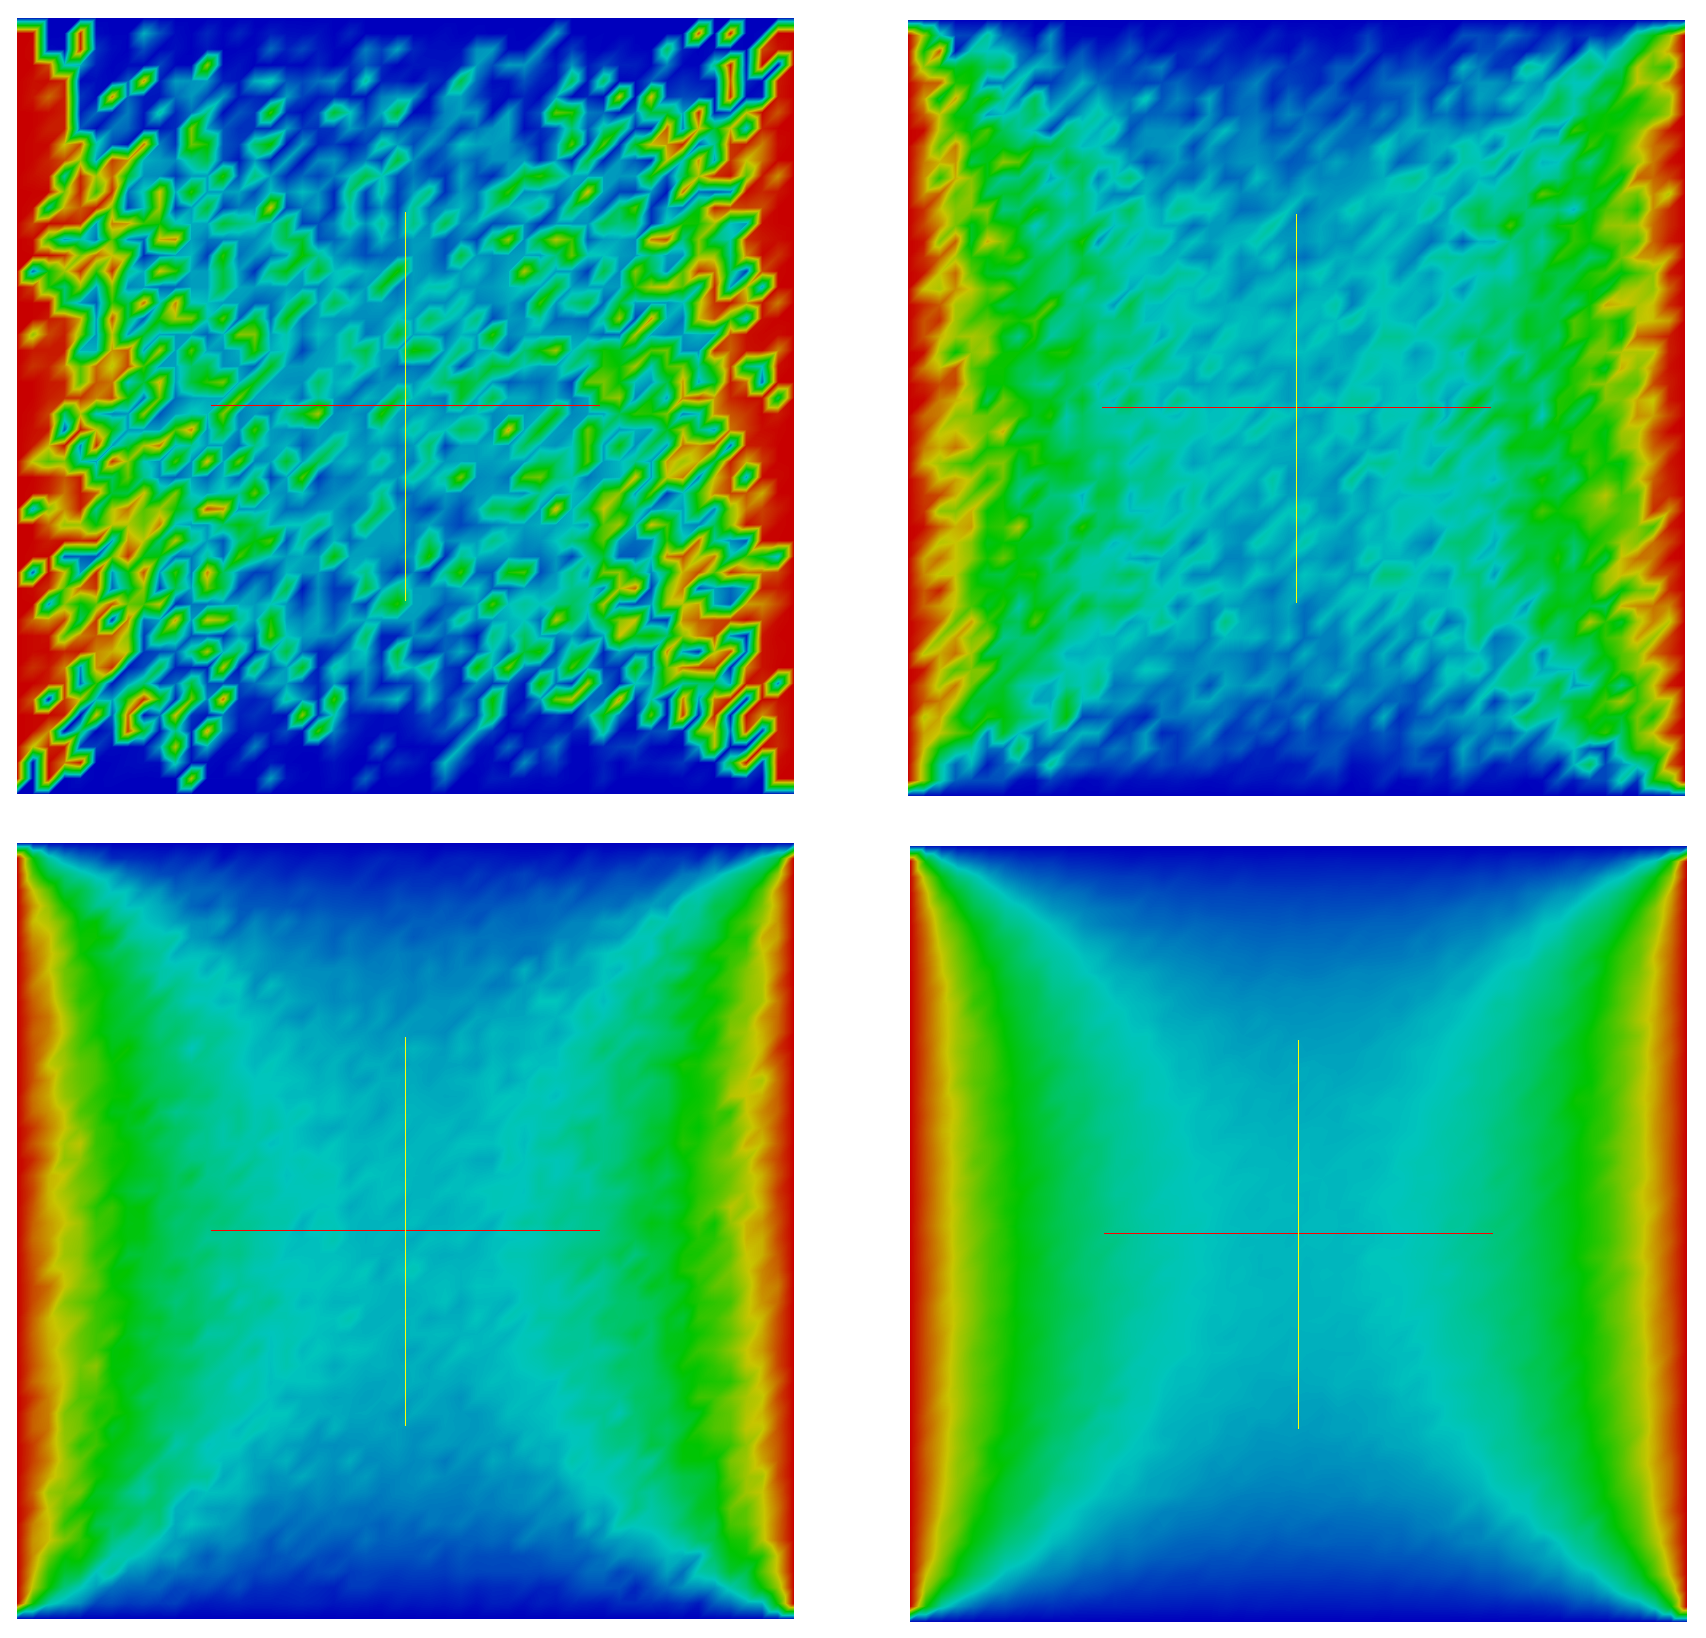
\includegraphics[width=6in]{chapters/mc_background/direct_evolution.png}
  \end{center}
  \caption{\textbf{Direct Monte Carlo solution to the heat equation
      with varying numbers of histories.} \textit{Top left: 1 history
      per state. Top right: 10 histories per state. Bottom left: 100
      histories per state. Bottom right: 1000 histories per state.}}
  \label{fig:direct_evolution}
\end{figure}
As the number of histories used per state is increased, the
statistical variance of the solutions is decreased as more tallies are
made. Starting with a single history at each state in the domain, the
high variance prevents a precise solution from being obtained although
we begin to see the solution take shape as expected. It is interesting
to note here that as the statistical uncertainty is reduced at each
grid point in the domain, the solution is resolved in a certain sense,
analogous to the convergence of a traditional iterative method.
\clearpage

\subsection{Adjoint Neumann-Ulam Method}
\label{sec:adjoint_mc}
An alternative to forward Monte Carlo matrix inversion is the adjoint
method. We begin by defining the linear system adjoint to
Eq~(\ref{eq:linear_problem}):
\begin{equation}
  \ve{A}^T \ve{y} = \ve{d}\:,
  \label{eq:adjoint_linear_problem}
\end{equation}
where $\ve{y}$ and $\ve{d}$ are the adjoint solution and source
vectors respectively and $\ve{A}^T$ is the adjoint operator for
$\ve{A} \in \mathbb{R}^{N \times N}$. We can split this equation to
mirror Eq~(\ref{eq:richardson_split}):
\begin{equation}
  \ve{y} = \ve{H}^T \ve{y} + \ve{d}\:.
  \label{eq:adjoint_split_system}
\end{equation}
As was required for convergence with the direct method using
Eq~(\ref{eq:richardson_split}), the spectral radius of $\ve{H}$ must
remain less than 1 as $\ve{H}^T$ contains the same eigenvalues and
therefore has the same spectral radius. By defining the following
adjoint inner product equivalence \cite{spanier_monte_1969}:
\begin{equation}
  \langle \ve{A}^T \ve{y}, \ve{x} \rangle = \langle \ve{y}, \ve{A}
  \ve{x} \rangle\:.
  \label{eq:adjoint_operator_product}
\end{equation}
it follows that:
\begin{equation}
  \langle \ve{x}, \ve{d} \rangle = \langle \ve{y}, \ve{b} \rangle\:.
  \label{eq:adjoint_vector_relation}
\end{equation}
Using these definitions, we can derive an estimator from the adjoint
method that will also give the solution vector, $\ve{x}$. As with the
direct method, we can acquire the adjoint solution by forming the
Neumann series by writing Eq~(\ref{eq:adjoint_split_system}) as:
\begin{equation}
  \ve{y} = (\ve{I} - \ve{H}^T)^{-1} \ve{d}\:,
  \label{eq:adjoint_split_system_2}
\end{equation}
which in turn yields the Neumann series using the adjoint operator:
\begin{equation}
  \ve{y} = \sum_{k=0}^{\infty} (\ve{H}^T)^k\ve{d}\:.
  \label{eq:adjoint_neumann_series}
\end{equation}
We expand this summation to again yield a series of transitions that
can be approximated by a Monte Carlo random walk sequence, this time
forming the Neumann series in reverse order:
\begin{equation}
  y_i = \sum_{k=0}^{\infty}\sum_{i_1}^{N}\sum_{i_2}^{N}\ldots
  \sum_{i_k}^{N}h_{i_k,i_{k-1}}\ldots h_{i_2,i_1} h_{i_1,i} d_{i_k}\:.
  \label{eq:adjoint_neumann_solution}
\end{equation}
We can readily build an estimator for the adjoint solution from this
series expansion, but we instead desire the solution to
Eq~(\ref{eq:linear_problem}). Here we have 2 unknowns, $\ve{y}$ and
$\ve{d}$, and therefore we require two constraints to close the
system. We use Eq~(\ref{eq:adjoint_vector_relation}) as the first
constraint and as a second constraint we select:
\begin{equation}
  \ve{d} = \boldsymbol{\delta}_j\:,
  \label{eq:adjoint_second_constraint}
\end{equation}
where $\boldsymbol{\delta}_j$ is one of a set of vectors in which the
$j^{th}$ component is the Kronecker delta function $\delta_{i,j}$. If
we apply Eq~(\ref{eq:adjoint_second_constraint}) to our first
constraint Eq~(\ref{eq:adjoint_vector_relation}), we get the following
convenient outcome:
\begin{equation}
  \langle \ve{y}, \ve{b} \rangle = \langle \ve{x},
  \boldsymbol{\delta}_j \rangle = x_j \:,
  \label{eq:inner_product_constraint}
\end{equation}
meaning that if we compute the inner product of the original source
and the adjoint solution using a delta function source, we recover one
component of the original solution.

In terms of radiation transport, this adjoint method is equivalent to
a traditional forward method where the initial state $i_0$ of the
random walk is determined by sampling the source vector $\ve{b}$ with
probabilities:
\begin{equation}
  P_{(i_0=i)}(\nu) = \frac{|b_i|}{||\ve{b}||_1}\:,
  \label{eq:adjoint_source_probability}
\end{equation}
with a random walk starting weight of:
\begin{equation}
  W_0 = ||\ve{b}||_1 \frac{b_i}{|b_i|}\:,
  \label{eq:adjoint_starting_weight}
\end{equation}
which gives the additional useful relation:
\begin{equation}
  b_{i_0} = W_0 P_{(i_0=i)}\:.
  \label{eq:adjoint_source_definition}
\end{equation}
As a result of using the adjoint system, we modify our probabilities
and weights using the \textit{adjoint Neumann-Ulam decomposition} of
$\ve{H}$:
\begin{equation}
  \ve{H}^{T} = \ve{P} \circ \ve{W}\:,
  \label{eq:adjoint_neumann_ulam}
\end{equation}
where now we are forming the decomposition with respect to the
transpose of $\ve{H}$. We then follow the same procedure as the direct
method for forming the probability and weight matrices in the
decomposition. Using the adjoint form, probabilities should instead be
column-scaled:
\begin{equation}
  p_{ij} = \frac{|h_{ji}|}{\sum_j |h_{ji}|}\:,
  \label{eq:adjoint_probability}
\end{equation}
such that we expect to select a new state, $j$, from the current state
in the random walk, $i$, by sampling column-wise (or row-wise if an
adjoint probability matrix is formed). Per
Eq~(\ref{eq:adjoint_neumann_ulam}), the transition weight is then
defined as:
\begin{equation}
  w_{ij} = \frac{h_{ji}}{p_{ij}}\:.
  \label{eq:adjoint_weight}
\end{equation}
Using the decomposition we can then define an expectation value for
the adjoint method. Given Eq~(\ref{eq:direct_permutation_weight}) as
the weight generated for a particular random walk permutation as in
Eq~(\ref{eq:mc_walk_permutation}) and our result from
Eq~(\ref{eq:inner_product_constraint}) generated by applying the
adjoint constraints, the contribution to the solution in state $j$
from a particular random walk permutation of $k$ events is then the
\textit{collision estimator}\footnote{The variance for this estimator
  is discussed in Appendix~\ref{chap:estimator_variance}.}:
\begin{equation}
  X_{j}(\nu) = \sum_{m=0}^k W_{m} \delta_{i_m,j}\:,
  \label{eq:adjoint_permutation_contribution}
\end{equation}
where the Kronecker delta indicates that the tally contributes only in
the current state, $i_m$, of the random walk.  Note here that the
estimator in Eq~(\ref{eq:adjoint_permutation_contribution}) does not
have a dependency on the source state as in
Eq~(\ref{eq:direct_permutation_contribution}), providing a remedy for
the situation in the direct method where we must start a random walk
in each source state for every permutation if we want to compute a
solution estimate for that state. In the adjoint method, we instead
tally in all states and those of lesser importance will not be visited
as frequently by the random walk. Finally, the expectation value using
all permutations is:
\begin{equation}
  E\{X_j\} = \sum_{\nu} P_{\nu} X_{j}(\nu)\:
  \label{eq:adjoint_expectation_value}
\end{equation}
which, if expanded in the same way as the direct method and utilizing
Eq~(\ref{eq:adjoint_source_definition}) to insert the source term,
directly recovers the exact solution:
\begin{equation}
  \begin{split}
    E\{X_j\} &=\sum_{k=0}^{\infty}\sum_{i_1}^{N}\sum_{i_2}^{N}\ldots
    \sum_{i_k}^{N} b_{i_0} p_{i_0,i_1}p_{i_1,i_2}\ldots
    p_{i_{k-1},i_k} w_{i_0,i_1}w_{i_1,i_2}\ldots
    w_{i_{k-1},i_k} \delta_{i_k,j} \\ &= x_{j}\:,
  \end{split}
  \label{eq:adjoint_expectation_expansion}
\end{equation}
therefore, also providing an unbiased Monte Carlo estimate of the
solution. It should be noted here that
Eq~(\ref{eq:adjoint_expectation_expansion}) only computes a single
component of our desired solution vector when really what we desire is
the entire solution vector. In an adjoint Monte Carlo simulation using
this estimator, the $w_{ij}$ elements that are added into the tally
for each state are only selected if/when the random walk currently
resides in that state. Much like a mesh tally in a particle transport
simulation, we have $N$ simultaneous tallies for $\ve{A} \in
\mathbb{R}^{N \times N}$ that will yield the entire solution vector.

Like the direct method, we also desire a criteria for random walk
termination for problems where only an approximate solution is
necessary. For the adjoint method, we utilize a \textit{relative
  weight cutoff}:
\begin{equation}
  W_f = W_c W_0\:,
  \label{eq:relative_weight_cutoff}
\end{equation}
where $W_c$ is defined as in the direct method. The adjoint random
walk will then be terminated after $m$ steps if $W_m < W_f$ as tally
contributions become increasingly small.

\subsubsection{Expected Value Estimator}
\label{subsec:expected_value_estimator}
In addition to the collision estimator, an additional estimator is
available due to the work of Okten \cite{okten_solving_2005} that uses
the method of expected values as a means to improve the Monte Carlo
estimate. As outlined by Spanier and Gelbard
\cite{spanier_monte_1969}, the method of expected values is a
deterministic averaging of events that may potentially occur in the
Monte Carlo random walk sequence. Okten applied this principle
directly to discrete Monte Carlo by forming the \textit{expected value
  estimator}\footnote{The variance for this estimator is discussed in
  Appendix~\ref{chap:estimator_variance}.} for a random walk of $k$
events:
\begin{equation}
  X_{j}(\nu) = b_j + \sum_{m=0}^k W_m h_{j,i_m}\,
  \label{eq:expected_value_estimator}
\end{equation}
where now the contribution of the iteration matrix is
deterministically averaged at step $m$ over all potential states $j$
that may be reached from the current state $i_m$. Via Okten, the
estimator can be shown to be unbiased through a comparison to the
collision estimator. We can first rewrite the summation in
Eq~(\ref{eq:expected_value_estimator}):
\begin{equation}
  X_{j}(\nu) = b_j + \sum_{m=0}^k \sum_{i=1}^N W_m
  \delta_{i_m,i} h_{ji}\,
  \label{eq:unbiased_eval_1}
\end{equation}
where $N$ is the number of states in the system. Immediately, we see
the collision estimator as defined by
Eq~(\ref{eq:adjoint_permutation_contribution}) and can therefore write
the expectation value as:
\begin{equation}
  E\{X_{j}\} = b_j + \sum_{i=1}^N E\{X_{i}\} h_{ji}\,
  \label{eq:unbiased_eval_2}
\end{equation}
which is equivalently is the $j^{th}$ component of
Eq~(\ref{eq:richardson_split}):
\begin{equation}
  E\{X_{j}\} = b_j + \sum_{i=1}^N x_{i} h_{ji}\,
  \label{eq:unbiased_eval_2}
\end{equation}
and is therefore an unbiased estimate. Compared to the collision
estimator, the expected value estimator provides additional
information at every step of the random walk, yielding potentially
better statistics with the same amount of transport
work. Conveniently, even if no Monte Carlo histories are computed, the
expected value estimator still deterministically computes the first
term of the Neumann Series, $\ve{H}^0\ve{b}$, whereas the collision
estimator will provide no information.

\subsubsection{Adjoint Method: Evolution of a Solution}
\label{subsec:adjoint_evolution}
As a means of visually demonstrating the adjoint Monte Carlo method,
again consider the 2-dimensional thermal diffusion problem with
sources on the left and right hand sides of the domain and a smaller
uniform source as shown in Figure~\ref{fig:heat_setup}. Using the
adjoint method with the collision estimator, the number of histories
sampled from the source was increased from 10 to 10,000,000 in order
to show its effects on the solution and the statistical nature of the
method. Figure~\ref{fig:adjoint_evolution} gives these results.
\begin{figure}[t!]
  \begin{center}
    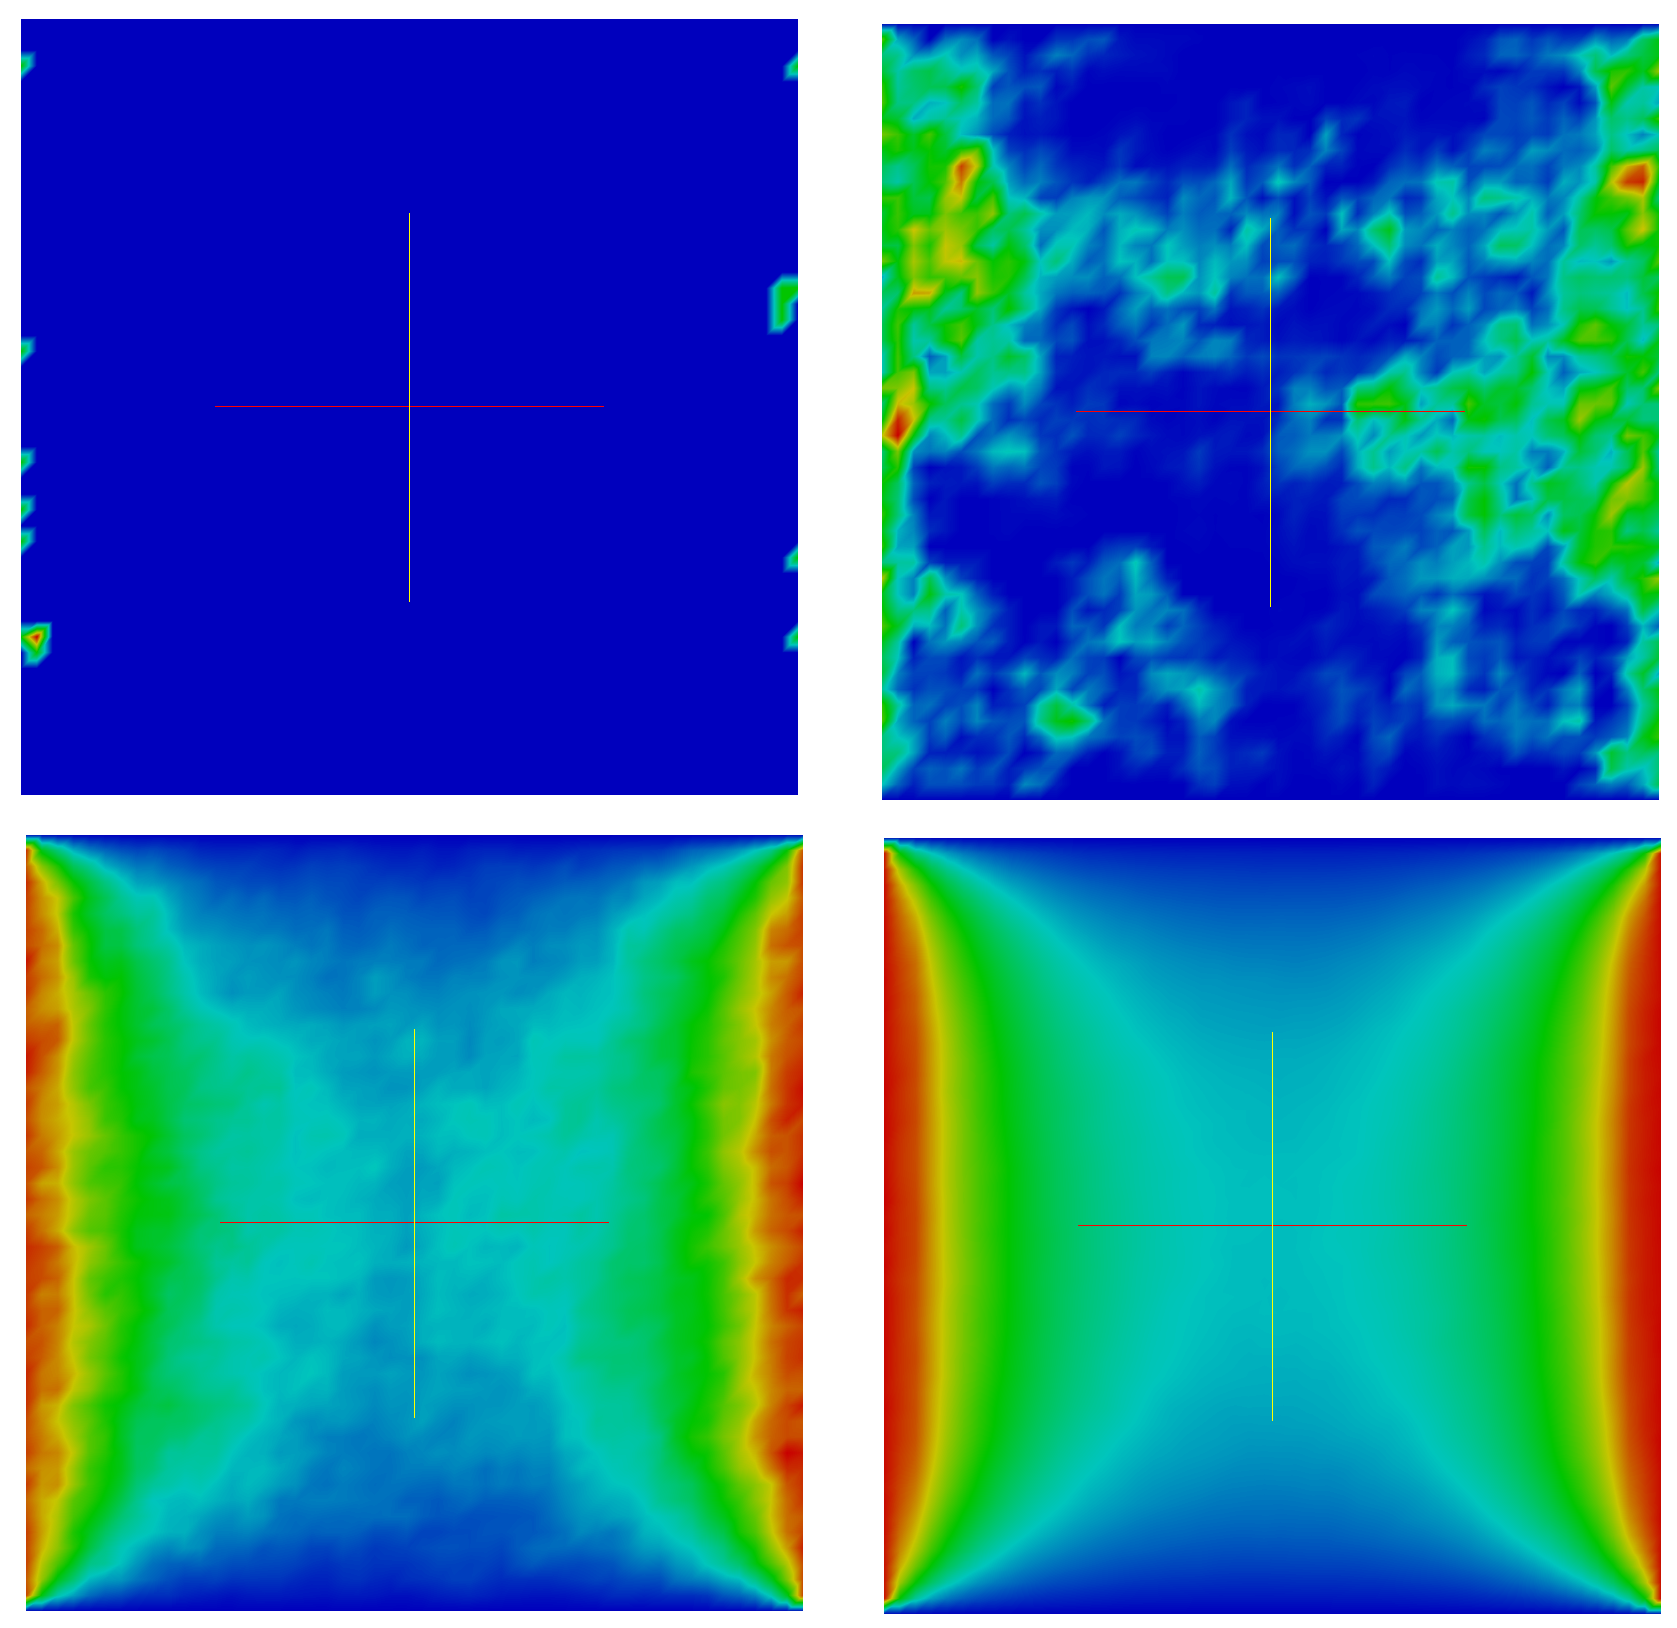
\includegraphics[width=6in]{chapters/mc_background/adjoint_evolution.png}
  \end{center}
  \caption{\textbf{Adjoint Monte Carlo solution to the heat equation
      with varying numbers of histories.} \textit{Top left: 10
      histories per state. Top right: 1,000 histories per
      state. Bottom left: 100,000 histories per state. Bottom right:
      10,000,000 histories per state.}}
  \label{fig:adjoint_evolution}
\end{figure}
As the number of histories used per state (or DOF) is increased, the
statistical variance of the solutions is decreased as more tally
contributions are made. At 10,000,000 histories per state, enough
information has been tallied to generate a reasonable estimate for the
structure of the solution. The visual difference between
Figures~\ref{fig:direct_evolution} and \ref{fig:adjoint_evolution} is
precisely that determined by their mathematics. As the adjoint
solution evolves with the addition of histories, more histories
emanate from the boundary the smaller uniform source in the domain
with more penetrating from the boundary into the domain and making
contributions to the tallies in those states as they are transported.

\clearpage

%%---------------------------------------------------------------------------%%
\section{Sequential Monte Carlo}
\label{sec:sequential_mc}
The direct and adjoint Neumann-Ulam methods described are limited by a
convergence rate of $1/\sqrt{N}$ by the Central Limit Theorem where
$N$ is the number of random walk permutations. In 1962, Halton
presented a residual Monte Carlo method that moves towards exponential
convergence rates \cite{halton_sequential_1962} and further refined
his work some years later \cite{halton_sequential_1994} with
applications of his work by the transport community confirming
exponential convergence rates \cite{evans_residual_2003}. Halton's
method, sequential Monte Carlo, utilizes the adjoint Monte Carlo
solver as a means of directly reducing the elements residual
vector. He proposed the following iterative scheme as a solution to
Eq~(\ref{eq:linear_problem})\:
\begin{subequations}
  \begin{gather}
    \ve{r}^k = \ve{b} - \ve{A}\ve{x}^k\:,\\  
    \ve{A}\boldsymbol{\delta}^{k} = \ve{r}^{k}\:,\\
    \ve{x}^{k+1} = \ve{x}^k + \boldsymbol{\delta}^{k}\:,
  \end{gather}
  \label{eq:sequential_monte_carlo}
\end{subequations}
where the correction $\boldsymbol{\delta}^k$ is computed by the
adjoint Monte Carlo method at each iteration. The merits of Halton's
approach are immediately visible in that we have now broken the
binding of the convergence rate to the Central Limit Theorem. Here,
the Monte Carlo solver is used to produce a correction from the
residual, analogous to using the residual to extract a correction from
the search subspace in a projection method. By doing this, the Monte
Carlo error is bound in the correction used to update the solution and
therefore does not explicitly manifest itself in the overall
convergence of the solution. The downside of such a method is that if
the solution guess is poor, then many iterations are required in order
to reach exponential converge as the Monte Carlo error (and therefore
the Central Limit Theorem) does dominate in this situation.

%%---------------------------------------------------------------------------%%
\section{Monte Carlo Synthetic Acceleration}
\label{sec:mcsa}
Using the ideas of Halton, Evans and Mosher recently developed a Monte
Carlo solution method that was not prohibited severely by the quality
of the initial guess for the system \cite{evans_monte_2009} and later
applied it more rigorously as a solution mechanism for the radiation
diffusion equation \cite{evans_monte_2012}. Their approach was instead
to use residual Monte Carlo as a synthetic acceleration for a
stationary method. To derive this method, we begin by splitting the
operator in Eq~(\ref{eq:linear_problem})
\begin{equation}
  \ve{x} = (\ve{I} - \ve{A})\ve{x} + \ve{b}\:.
  \label{eq:linear_split}
\end{equation}
With this we can then define the stationary method
\textit{Richardson's iteration} as:
\begin{equation}
  \ve{x}^{k+1} = (\ve{I} - \ve{A})\ve{x}^k + \ve{b}\:,
  \label{eq:richardsons_iteration}
\end{equation}
which will converge if $\rho(\ve{I} - \ve{A}) < 1$. We then define the
solution error at the $k^{th}$ iterate relative to the true solution:
\begin{equation}
  \delta \ve{x}^k = \ve{x} - \ve{x}^k\:.
  \label{eq:mcsa_error}
\end{equation}
Subtracting Eq~(\ref{eq:richardsons_iteration}) from
Eq~(\ref{eq:linear_split}) we get:
\begin{equation}
  \delta \ve{x}^{k+1} = (\ve{I} - \ve{A})\delta \ve{x}^k\:.
  \label{eq:mcsa_setup_1}
\end{equation}
Subtracting from this $(\ve{I} - \ve{A})\delta \ve{x}^{k+1}$ yields:
\begin{equation}
  \begin{split}
    \ve{A}\delta \ve{x}^{k+1} &= (\ve{I} -
    \ve{A})(\ve{x}^{k+1}-\ve{x}^{k}) \\ &= \ve{r}^{k+1}\:.
    \label{eq:mcsa_setup_2}
  \end{split}
\end{equation}
Using this, we define the following scheme that will converge in one
iteration if $\ve{A}$ is inverted exactly:
\begin{subequations}
  \begin{gather}
    \ve{x}^{k+1} = (\ve{I} - \ve{A})\ve{x}^k + \ve{b}\:,\\
    \ve{A} \delta \ve{x}^{k+1} = \ve{r}^{k+1}\:,\\
    \ve{x} = \ve{x}^{k+1} + \delta \ve{x}^{k+1}\:.
  \end{gather}
  \label{eq:mcsa_setup_3}
\end{subequations}
However, $\ve{A}$ is only approximately inverted by our numerical
methods and therefore we instead pose an iterative scheme in which the
Monte Carlo solvers are used to invert the operator. The
\textit{Fixed-Point Monte Carlo Synthetic Acceleration} (MCSA) method
is defined as:
\begin{subequations}
  \begin{gather}
    \ve{x}^{k+1/2} = \ve{x}^k + \ve{r}^k\:,\\
    \ve{r}^{k+1/2} = \ve{b} - \ve{A}\ve{x}^{k+1/2}\:,\\
    \ve{A}\delta\ve{x}^{k+1/2} = \ve{r}^{k+1/2}\:,\\
    \ve{x}^{k+1} = \ve{x}^{k+1/2} + \delta \ve{x}^{k+1/2}\:,\\
    \ve{r}^{k+1} = \ve{b} - \ve{A}\ve{x}^{k+1}\:,
  \end{gather}
  \label{eq:mcsa}
\end{subequations}
where a Neumann-Ulam Monte Carlo method is used to generate the
solution correction from the residual and Richardson's iteration in
the first step has been rewritten as a residual correction. Using
Monte Carlo in this way achieves the same effect as Halton's method,
decoupling its convergence rate from the overall convergence rate of
the method. Here, the approximate Monte Carlo solution is not driven
to a particular convergence as it merely supplies a correction for the
initial guess generated by Richardson's iteration. Rather, only a set
number of histories are required using the Neumann-Ulam method to
generate the correction. In addition, the fact that the scheme in
Eq~(\ref{eq:mcsa_setup_3}) will converge in one iteration if $\ve{A}$
is inverted exactly means that as more and more stochastic histories
are used to compute the correction and the error is reduced towards
zero, the number of iterations required for MCSA to converge should
decrease accordingly, thus accelerating the solution.

In addition to the Monte Carlo solver parameters dictating the number
of histories and weight cutoff, the outer MCSA iterations also have
the following stopping criteria:
\begin{equation}
  ||\ve{r}||_\infty < \epsilon \ ||\ve{b}||_\infty\:,
  \label{eq:mcsa_stopping_criteria}
\end{equation}
where $\epsilon$ is a user-defined parameter. As with any iterative
method, other stopping criteria using other vector norms could be
computed, however, for this work we will only use
Eq~(\ref{eq:mcsa_stopping_criteria}). We therefore have 3 parameters
to tune in an MCSA implementation: the number of Monte Carlo histories
computed in the Neumann-Ulam solve during each MCSA iteration, the
weight cutoff for those histories, and the total MCSA convergence
tolerance as specified by $\epsilon$.

\subsection{Alternative Fixed Point Iterations}
\label{subsubsec:alternative_fixed_point}
In addition to the basic Richardson iteration, the MCSA algorithm
presented in Eq~(\ref{eq:mcsa}) can be used to accelerate any fixed
point iteration which only depends on the state (typically the
residual) of the last iteration. As outlined in
Appendix~\ref{ch:linear_problem}, subspace methods take on a general
form using the Petrov-Galerkin conditions as constraints for
extracting a correction from the search subspace as given by
Eq~(\ref{eq:linear_projection_iteration}). Those that are
one-dimensional may be used with fixed-point MCSA as they only depend
the previous iteration for information. As an example, for
positive-definite but not necessarily symmetric problems, the minimal
residual iteration \cite{saad_iterative_2003} can be used in
conjunction with MCSA where the residual vector, $\mathbf{r}$, defines
the search subspace and the action of the linear operator on the
residual vector, $\mathbf{A}\mathbf{r}$, defines the constraint
subspace. Using this, we can then define an MCSA scheme that
accelerates the minimal residual iteration:
\begin{subequations}
  \begin{gather}
    \alpha = \frac{\langle \mathbf{A}\mathbf{r}^k, \mathbf{r}^k
      \rangle}{\langle \mathbf{A}\mathbf{r}^k, \mathbf{A}\mathbf{r}^k
      \rangle}\:, \\
    \ve{x}^{k+1/2} = \ve{x}^k + \alpha \ve{r}^k\:,
    \label{eq:min_res_correction}\\
    \ve{r}^{k+1/2} = \ve{b} - \ve{A}\ve{x}^{k+1/2}\:,\\ 
    \ve{A}\delta\ve{x}^{k+1/2} = \ve{r}^{k+1/2}\:,\\ 
    \ve{x}^{k+1} = \ve{x}^{k+1/2} + \delta\ve{x}^{k+1/2}\:,\\ 
    \ve{r}^{k+1} = \ve{b} - \ve{A}\ve{x}^{k+1}\:.
  \end{gather}
  \label{eq:mcsa_min_res}
\end{subequations}
where $\alpha$ is an optimal extrapolation parameter generated from
the constraints. Interestingly, this scheme is nearly identical to the
Richardson iteration version in Eq~(\ref{eq:mcsa}) except now the
additional extrapolation parameter, $\alpha$, is applied to the
residual correction in Eq~(\ref{eq:min_res_correction}) as a means of
selecting a more optimal search direction at each iteration,
potentially further improving convergence.

\subsection{Preconditioning MCSA}
\label{subsec:stochastic_preconditioning}
In most cases, at least a minimal amount of \textit{preconditioning}
of the linear system will be required in order to use the class of
stochastic methods described. Although these methods have no symmetry
requirements for convergence, they do require that the spectral radius
of the iteration matrix be less than one. Preconditioning serves as a
means of achieving this by altering the eigenvalue spectrum of the
iteration matrix.

\subsubsection{Basic Preconditioning}
\label{subsubsec:basic_mcsa_preconditioning}
As an example of basic preconditioning, to achieve a spectral radius
of less than one for diagonally dominant matrices point Jacobi
preconditioning can be used such that the preconditioning matrix
$\ve{M}$ is:
\begin{equation}
  \ve{M} = diag(\ve{A})\:,
  \label{eq:jacobi_preconditioner}
\end{equation}
which may be trivially inverted. With the application of this
preconditioner we are instead solving the following scaled linear
system:
\begin{equation}
  \ve{M}^{-1}\ve{A}\ve{x} = \ve{M}^{-1}\ve{b}\:.
  \label{eq:jacobi_precond_linear_problem}
\end{equation}
Next, we can apply MCSA to solve
Eq~(\ref{eq:jacobi_precond_linear_problem}): 
\begin{subequations}
  \begin{gather}
    \ve{x}^{k+1/2} = \ve{x}^k +
    \ve{M}^{-1}\ve{r}^k\:,\\ \ve{r}^{k+1/2} =
    \ve{b}-\ve{A}\ve{x}^{k+1/2}\:,\\ \ve{M}^{-1}\ve{A}\delta\ve{x}^{k+1/2}
    = \ve{M}^{-1}\ve{r}^{k+1/2}\:,\\ \ve{x}^{k+1} = \ve{x}^{k+1/2} +
    \delta \ve{x}^{k+1/2}\:,\\
    \ve{r}^{k+1} = \ve{b} - \ve{A}\ve{x}^{k+1}\:,
    \label{eq:jacobi_preconditioned_mcsa}
  \end{gather}
\end{subequations}
where the Neumann-Ulam Monte Carlo solve now has a preconditioned
operator from which to build weights and probabilities for transport
and a preconditioned source vector to sample.

Choosing point Jacobi preconditioning with MCSA is advantageous for
several reasons. First, $\rho(\ve{I} - \ve{M}^{-1}\ve{A}) < 1$ is true
for all $\ve{A}$ that is diagonally dominant and is easy to formulate
because the inversion of $\ve{M}$ is trivial. Second, because the
Monte Carlo method used within MCSA to compute the correction operates
on a linear problem with the preconditioned operator, then $\ve{H}$ in
the Neumann-Ulam solver will have a zero term in each of its diagonal
elements, thereby eliminating all in-state transitions during the
random walk sequence. Because of this, point Jacobi preconditioning
should be considered for many classes of problems, regardless of any
other preconditioning that is applied to the system. In addition,
Jacobi preconditioning has been shown to be an effective
preconditioning mechanism for MCSA when used with the thermal
radiation diffusion equation \cite{evans_monte_2012}.

\clearpage

\subsubsection{General Preconditioning Strategies}
\label{subsubsec:general_mcsa_preconditioning}
It is possible to use general left, right, and left/right
preconditioning with MCSA by carefully considering the underlying
Monte Carlo problem that will be solved with the Neumann-Ulam
method. We consider here the general left/right preconditioned method
as the left or right preconditioned methods can be inferred from its
formulation. We consider a left preconditioner $\ve{M_L}$ and a right
preconditioner $\ve{M_R}$. The left/right preconditioned linear
problem is then:
\begin{equation}
  \ve{M}_L^{-1}\ve{A}\ve{M}_R^{-1}\ve{M}_R\ve{x} = \ve{M}_L^{-1}\ve{b}\:.
  \label{eq:left_right_linear_problem}
\end{equation}
To handle the right preconditioning, the system is written with a
substitution of variables:
\begin{equation}
  \ve{M}_L^{-1}\ve{A}\ve{M}_R^{-1}\ve{u} = \ve{M}_L^{-1}\ve{b}\:,
  \label{eq:left_right_subs_problem}
\end{equation}
with
\begin{equation}
  \ve{x} = \ve{M}_R^{-1}\ve{u}\:.
  \label{eq:left_right_recover}
\end{equation}
To apply such a method to MCSA, we solve for the substituted variable
$\ve{u}$ during the iteration sequence:
\begin{subequations}
  \begin{gather}
    \ve{u}^{k+1/2} = \ve{u}^k + \ve{r}^k\:,\\
    \ve{r}^{k+1/2} = \ve{M}_L^{-1}(\ve{b}-\ve{A}\ve{M}_R^{-1}\ve{u}^{k+1/2})\:,\\ 
    \ve{M}_L^{-1}\ve{A}\ve{M}_R^{-1}\delta\ve{u}^{k+1/2} = \ve{r}^{k+1/2}\:,\\ 
    \ve{u}^{k+1} = \ve{u}^{k+1/2} + \delta \ve{u}^{k+1/2}\:,\\
    \ve{r}^{k+1} = \ve{M}_L^{-1}(\ve{b}-\ve{A}\ve{M}_R^{-1}\ve{u}^{k+1})\:,
  \end{gather}
  \label{eq:left_right_mcsa}
\end{subequations}
and then recover the original solution vector with
Eq~(\ref{eq:left_right_recover}) after convergence. For the Monte
Carlo problem, we isolate the generation of the correction:
\begin{equation}
  \ve{M}_L^{-1}\ve{A}\ve{M}_R^{-1}\delta\ve{u}^{k+1/2} = \ve{r}^{k+1/2}\:,
  \label{eq:left_right_correction}
\end{equation}
and note that the preconditioned residual of the substituted variable
is now serving as the source and the new iteration matrix is:
\begin{equation}
  \ve{H} = \ve{I} - \ve{M}_L^{-1}\ve{A}\ve{M}_R^{-1}\:.
  \label{eq:left_right_iteration_matrix}
\end{equation}
As we require $(i,j)$ element-wise access to the iteration matrix in
order to construct probabilities and weights for the Monte Carlo
procedure from the Neumann-Ulam decomposition, the \textit{composite
  operator}, $\ve{M}_L^{-1}\ve{A}\ve{M}_R^{-1}$, must be formed via
matrix-matrix multiplication. 

Several possible shortcomings of this preconditioning approach are
readily observed. First, the matrix-matrix multiplication operation
for sparse, parallel distributed matrices is significantly more
expensive than a matrix-vector multiplication operation. Second, each
preconditioner must be explicitly inverted, an operation in itself
that may be expensive and which prohibits the use of any
preconditioners which provide no mechanism to extract their
inverse. Third, for many modern preconditioning methods, this
inversion may yield dense matrices, destroying sparsity and further
impeding the performance of a matrix-matrix multiplication
operation. It is also interesting to note that the Monte Carlo problem
in the general left/right preconditioned scheme given by
Eq~(\ref{eq:left_right_correction}) is not fully left/right
preconditioned (meaning that we do not recover $\ve{x}$), but instead
part of a sequence for finding the substituted variable $\ve{u}$. We
do, however, gain the benefits of this general preconditioning by
building the iteration matrix in
Eq~(\ref{eq:left_right_iteration_matrix}) from the fully
preconditioned linear operator. In addition, for MCSA to apply to
increasingly difficult problems, more advanced preconditioning
techniques that require the generation of the composite operator may
be necessary for convergence.

%%---------------------------------------------------------------------------%%
\section{Monte Carlo Synthetic Acceleration Analysis}
\label{sec:mcsa_analysis}
In this section we analyze the effects of various MCSA parameters to
better our understanding of the algorithm and facilitate future
work. In addition, we demonstrate the effectiveness of MCSA as
compared to Halton's Sequential Monte Carlo method. To do this, we
choose the two-dimensional time-dependent Poisson equation as a simple
model transport problem\footnote{The Poisson equation is a simple form
  of the diffusion equation and has a similar elliptic character in
  its time-dependent form to the neutron transport equations that will
  be solved in the next chapter.}:
\begin{equation}
  \frac{\partial \ve{u}}{\partial t} = \nabla^2 \ve{u}\:.
  \label{eq:poisson_equation}
\end{equation}
For all comparisons, a single time step is computed with backwards Euler time
integration. The Laplacian is differenced on a square Cartesian grid with a
second-order five-point stencil,
\begin{equation}
  \nabla^2_5 = \frac{1}{\Delta^2}[u_{i-1,j} + u_{i+1,j} + u_{i,j-1} +
    u_{i,j+1} - 4 u_{i,j}]\:,
  \label{eq:five_point_stencil}
\end{equation}
and a fourth-order nine-point stencil,
\begin{multline}
  \nabla^2_9 = \frac{1}{6\Delta^2}[4 u_{i-1,j} + 4 u_{i+1,j} + 4
    u_{i,j-1} + 4 u_{i,j+1} + u_{i-1,j-1}\\ + u_{i-1,j+1} +
    u_{i+1,j-1} + u_{i+1,j+1} - 20 u_{i,j}]\:,
  \label{eq:nine_point_stencil}
\end{multline}
both assuming a grid size of $\Delta$ in both the $i$ and $j$ directions. For
a single time step solution, we then have the following sparse linear system
to be solved with the MCSA method:
\begin{equation}
  \ve{A} \ve{u}^{n+1} = \ve{u}^n\:.
  \label{eq:poisson_eq_lin_sys}
\end{equation}
Both the stencils will be used to vary the size and density of the sparse
linear system in Eq.~(\ref{eq:poisson_eq_lin_sys}).

\subsection{Monte Carlo Method Selection}
\label{sec:mc_method_selection}
The MCSA method defined in Eq.~(\ref{eq:mcsa}) uses the adjoint method
to estimate the error in a residual Monte Carlo solve instead of the
direct method outlined in \S\ref{sec:direct_mc}. To demonstrate the
effectiveness of the adjoint method over the direct method within the
context of MCSA, we solve Poisson equation in a series of numerical
experiments. A timing and convergence study is used to demonstrate
the effectiveness of the adjoint method with the collision estimator
as compared to the direct method. To assess both the CPU time and
number of iterations required to converge to a solution, a problem of
constant $\Delta$ was used with varying values of the number of mesh
elements, fixing the spectral radius of the system at a constant value
for each variation. Both the five-point and nine-point stencils were
used with both the direct and adjoint solvers. For each case, $N
\times N$ total random walk permutations were computed per MCSA
iteration where $N \times N$ is the number of discrete grid points (or
degrees of freedom) in the system. Solver parameters were set to a
weight cutoff of \sn{1}{-4} for the stochastic linear solver and a
convergence tolerance of \sn{1}{-8} for the MCSA iterative solver.
Figure~\ref{fig:poisson_cpu_time} gives the CPU time needed for each
case to converge in seconds, and Figure~\ref{fig:poisson_iterations}
gives the number of iterations needed for each case to converge to the
specified tolerance, both as a function of the problem size. All
computations presented in this section and the remaining sections of
this chapter were completed on a 3.0 GHz Intel Core 2 Quad Q9650 CPU
machine with 16 GB 1067 MHz DDR3 memory.

\begin{figure}[t!]
  \centering
  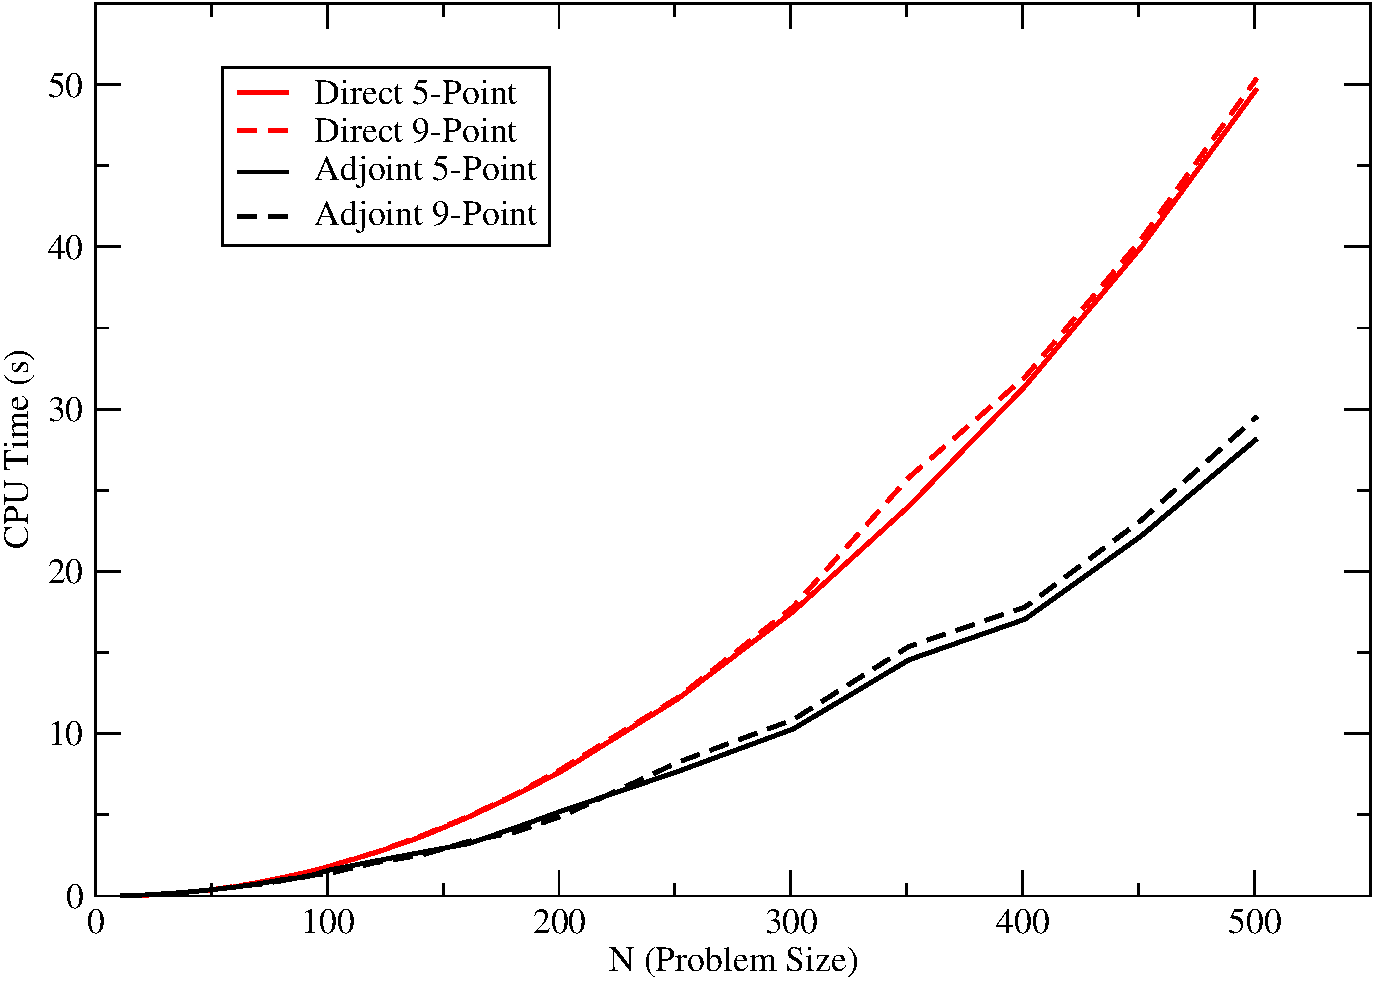
\includegraphics[width=5in,clip]{chapters/mc_background/dir_adj_cpu.pdf}
  \caption{\textbf{CPU Time (s) to converge vs. Problem Size ($N$ for
      an $N \times N$ square mesh).} \textit{Both the adjoint and
      direct solvers are used with the five point and nine point
      stencils. A CPU time speedup is noted with the adjoint method
      due to the higher density of random walk events in regions with
      a large residual.}}
  \label{fig:poisson_cpu_time}
\end{figure}

\begin{figure}[t!]
  \centering
  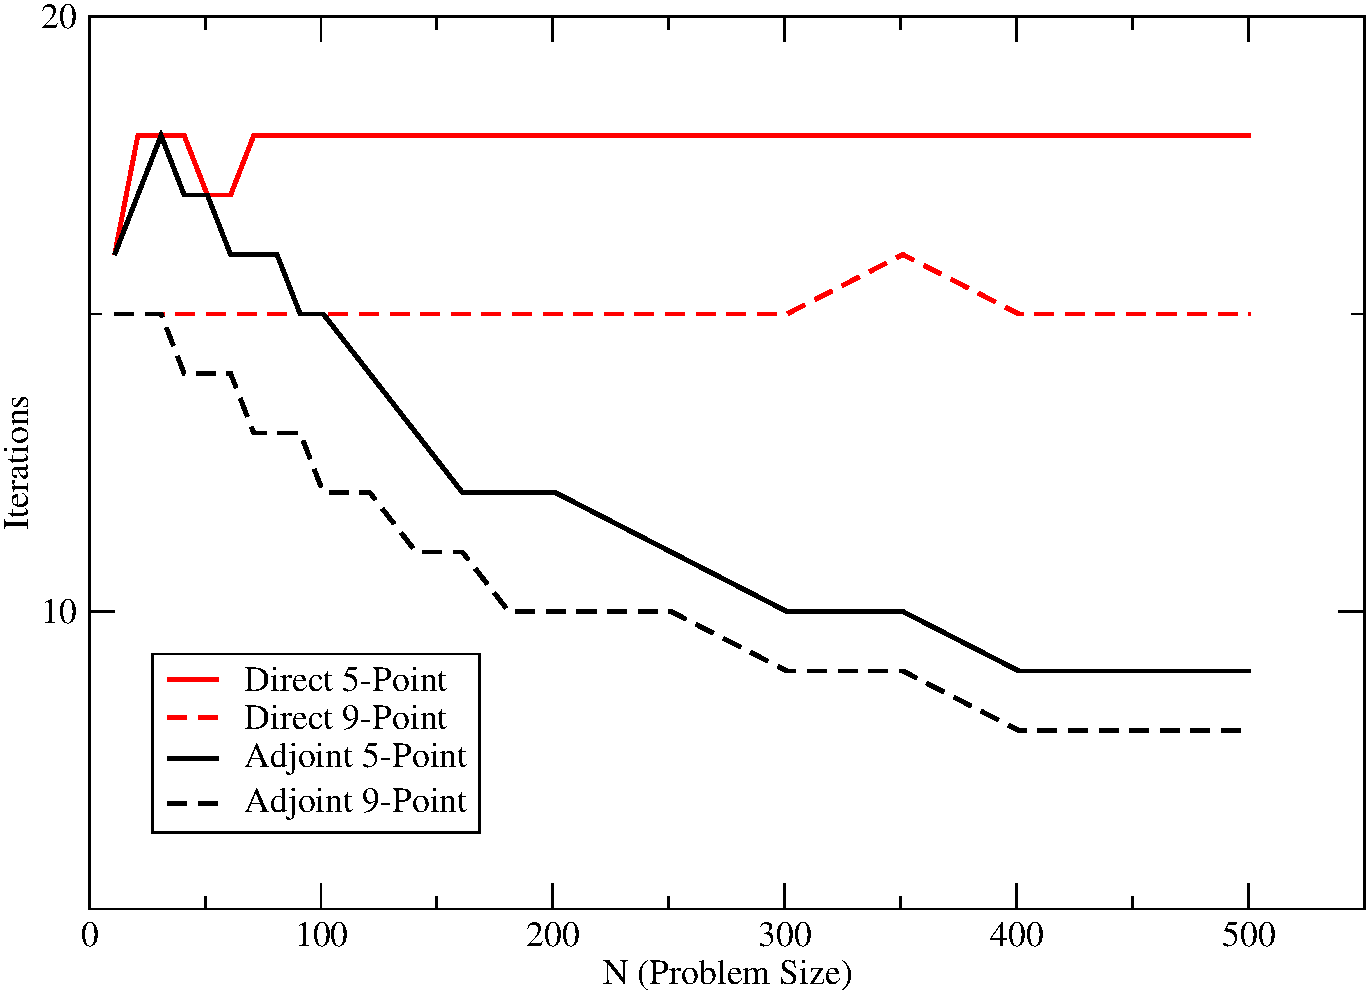
\includegraphics[width=5in,clip]{chapters/mc_background/dir_adj_iterations.pdf}
  \caption{\textbf{Iterations to converge vs. Problem Size ($N$ for an
      $N \times N$ square mesh).} \textit{Both the adjoint and direct
      solvers are used with the five-point and nine-point stencils.}}
  \label{fig:poisson_iterations}
\end{figure}

We see clearly in Figure~\ref{fig:poisson_cpu_time} that the using the
adjoint solver with MCSA results in a speedup over the direct solver
while the number of iterations required to converge is also reduced as
shown in Figure~\ref{fig:poisson_iterations}. We expect this for
several reasons. First, with an equivalent number of histories
specified for both solvers per MCSA iteration and a system of size $N
\times N$, the direct solver will compute a single random walk for
each state in the system per iteration to acquire a solution in that
state. This is necessary in the direct method to ensure a contribution
from each state as the random walk sequence will only contribute to
the starting state. For the adjoint method, a total of $N \times N$
random walk events will have their starting state determined by
sampling the residual vector. Because the random walk sequence
contributes to the state in which it currently resides, sampling the
residual vector as the Monte Carlo source gives a higher density of
random walk events in regions with a high residual, thus giving a more
accurate correction in that region due to reduced statistical
error. 

From an iteration perspective, Figure~\ref{fig:poisson_iterations}
shows that using the direct method yields a roughly unchanging number
of iterations required to converge as the problem size
increases. Again, if we desire a correction value for all states in
the problem, then we must start a random walk in each state in the
system without taking into account the structure of the residual
vector. Because of this, as the problem size grows adding histories is
ineffective as many are added in states where the error is smaller
than in other parts of the problem, ultimately not reducing the number
of iterations needed to converge. Conversely, as the problem size
grows in the adjoint method, the additional stochastic histories that
will be computed are concentrated in regions with a large residual,
further reducing the stochastic error in the correction in those
regions and subsequently reducing the required number of iterations to
converge.

As an additional comparison, the convergence behavior of MCSA can be
analyzed using both the adjoint and direct solvers to detect any
performance benefits. To assess the convergence properties of MCSA
using each solver and stencil, the infinity norm of the residual
computed in Eq.~(\ref{eq:mcsa}) was collected at each iteration for a
fixed problem size of $N=500$. Figure~\ref{fig:poisson_convergence}
gives the results of these computations. We note that using the
adjoint method with the same number of stochastic histories per MCSA
iteration gives a faster rate of converge for the same reasons as
above. We also note here that fewer iterations are required for
convergence when the 9-point stencil is used to discretize the
Laplacian operator (although at no gain in speed as given by the
results in Figure~\ref{fig:poisson_cpu_time}). This is due to the fact
that the smaller discretization error directly corresponds to a more
well defined residual source generated by the Richardson extrapolation
for the Monte Carlo calculation. In addition, the better defined
source is transported through a domain described more accurately by
the 9-point stencil, thus yielding a more accurate correction vector
from the Monte Carlo calculation.

\begin{figure}[t!]
  \centering
  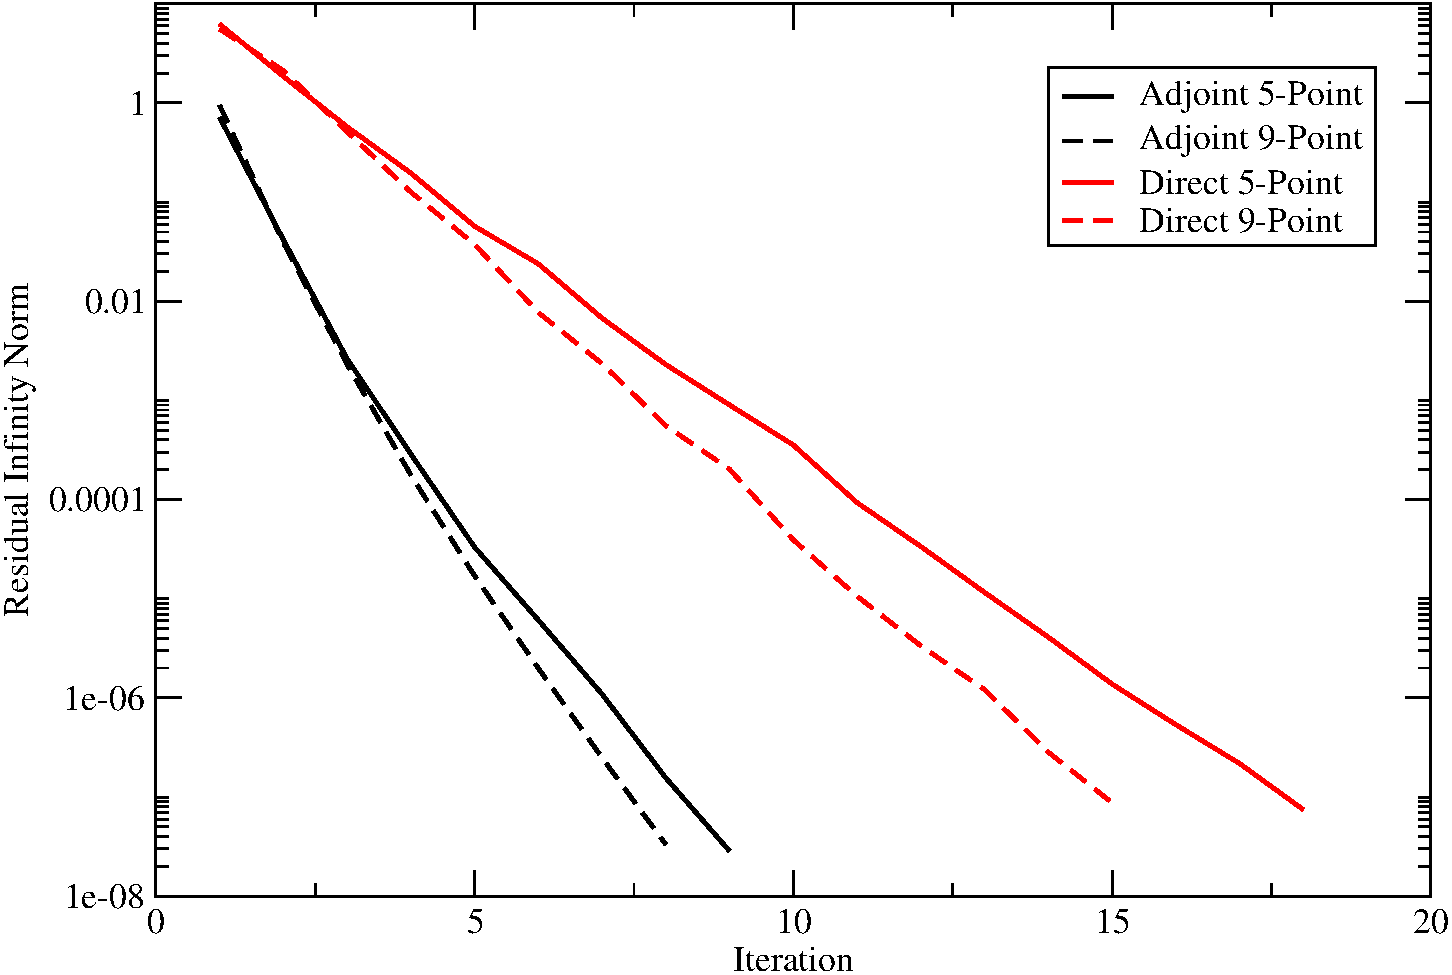
\includegraphics[width=5in,clip]{chapters/mc_background/dir_adj_conv.pdf}
  \caption{\textbf{Infinity norm of the solution residual
      vs. iteration number for a problem of size $N=500$.}
    \textit{Both the adjoint and direct solvers are used with the five
      point and nine point stencils. A higher rate of convergence is
      observed for MCSA using the adjoint Monte Carlo solver as
      compared to the direct method when both solvers compute the same
      number of random walks per iteration.}}
  \label{fig:poisson_convergence}
\end{figure}

\subsection{MCSA Comparison to Sequential Monte Carlo}
\label{subsec:sequential_comparison}
To further motivate using Monte Carlo Synthetic Acceleration, we
compare its performance to Halton's Sequential Monte Carlo. For this
comparison, we use the same transient Poisson problem as described in
the previous section and choose only the 5-point stencil to discretize
the Laplacian operator as the previous results yielded little
qualitative difference between the discretizations. Both MCSA and
Halton's method are used with the adjoint Monte Carlo solver and the
collision estimator. In order to complete the same study as in the
previous section, the number of histories computed by the Monte Carlo
solver at each iteration had to be doubled to $2 \times N \times N$ in
order to ensure convergence in Sequential Monte Carlo Method. For the
majority of the problems in the previous section, the Sequential
method used with $N \times N$ histories would not converge.

Figure~\ref{fig:seq_cpu_time} gives the CPU time results for this
comparison as a function of problem size while
Figure~\ref{fig:seq_iterations} gives the number of iterations to
converge as a function of problem size with a convergence tolerance of
\sn{1}{-8}. In both cases, using the Monte Carlo solver as a synthetic
acceleration rather than in a pure residual Monte Carlo scheme
resulted in a reduction in both CPU time and iterations required to
converge. The additional Richardson extrapolation between each Monte
Carlo solve in the MCSA method gives a better converged residual
source to use with the Monte Carlo calculation while the Sequential
method requires more iterations to achieve the same level of
convergence in the residual.

\begin{figure}[t!]
  \centering
  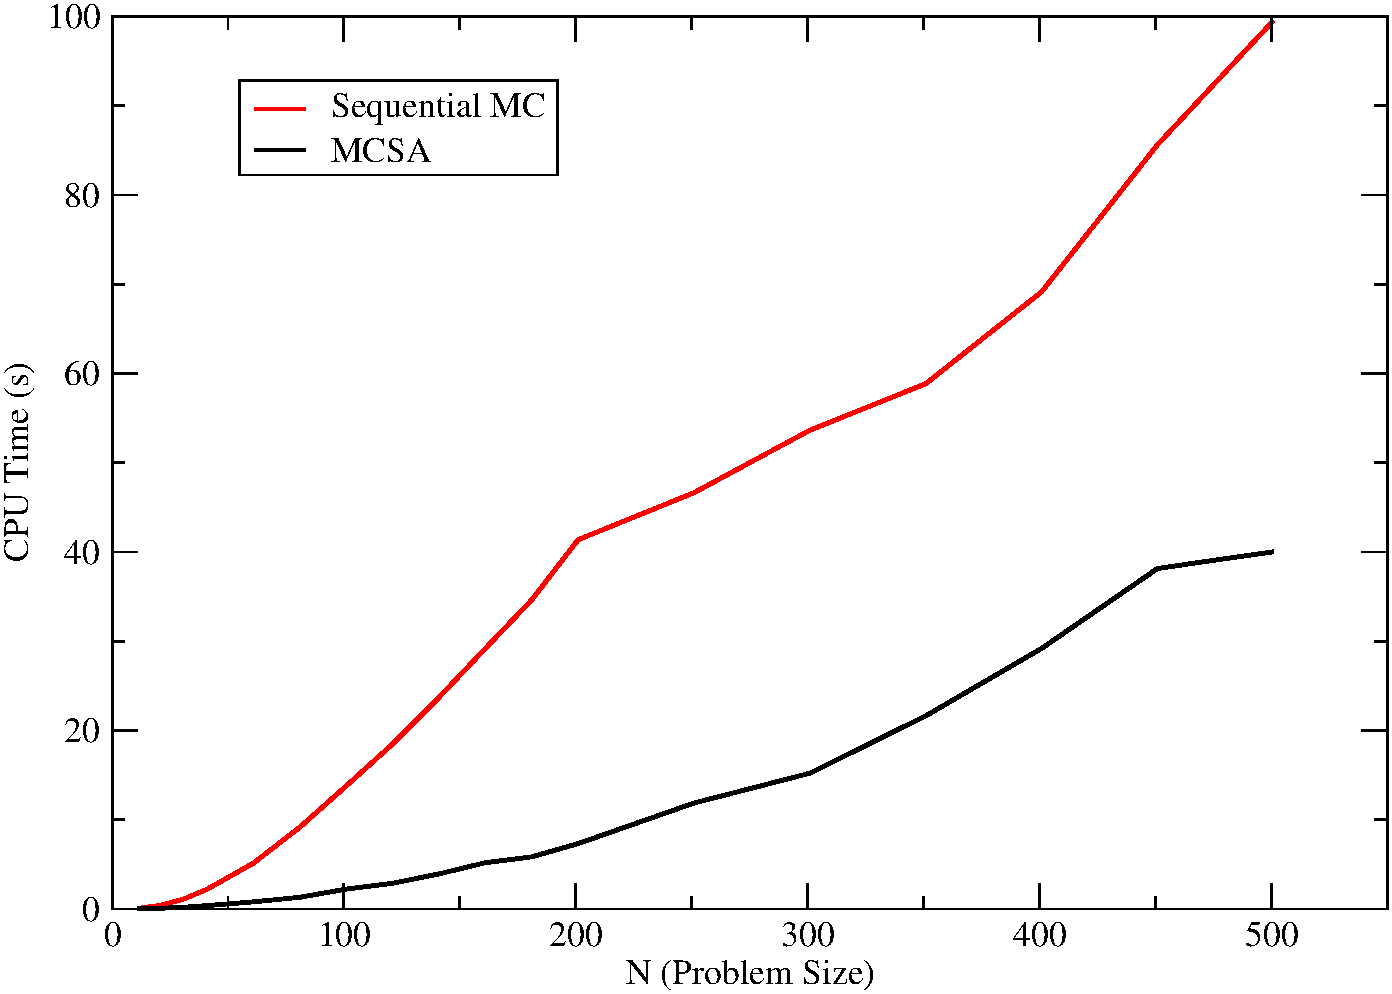
\includegraphics[width=4.5in,clip]{chapters/mc_background/seq_cpu.pdf}
  \caption{\textbf{CPU Time (s) to converge vs. Problem Size ($N$ for
      an $N \times N$ square mesh).} \textit{Both the Sequential Monte
      Carlo and MCSA solvers are used with the five point stencils and
      the adjoint Monte Carlo solver. The number of random walks was
      twice the number of discrete states in the system in order to
      ensure convergence in the Sequential Monte Carlo method.}}
  \label{fig:seq_cpu_time}
\end{figure}

\begin{figure}[t!]
  \centering
  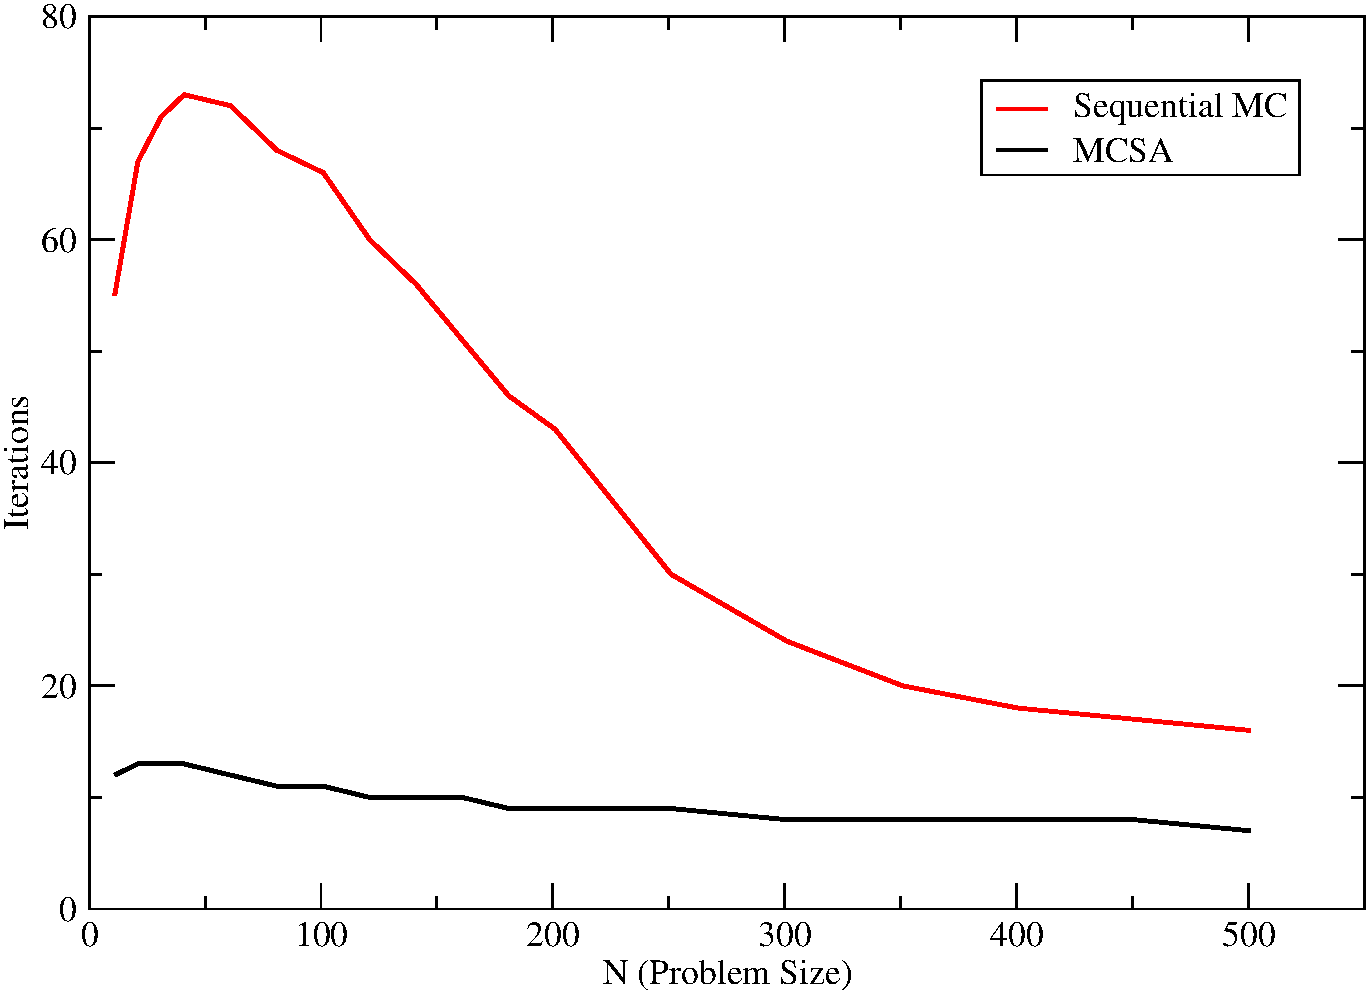
\includegraphics[width=4.5in,clip]{chapters/mc_background/seq_iterations.pdf}
  \caption{\textbf{Iterations to converge vs. Problem Size ($N$ for an
      $N \times N$ square mesh).} \textit{Both the Sequential Monte
      Carlo and MCSA solvers are used with the five point stencils and
      the adjoint Monte Carlo solver.}}
  \label{fig:seq_iterations}
\end{figure}

The benefits of using a synthetic acceleration scheme are also noted
when the infinity norm of the residual computed at each iteration for
both methods was collected at each iteration for a fixed problem sizes
of $N=100$ and $N=500$ as shown in figures Figure~\ref{fig:seq_100}
and \ref{fig:seq_500} respectively. In both cases, the Sequential
method is subject to two regimes of exponential convergence with high
frequency error modes removed in the first regime leaving lower
frequency and slower converging error modes in the second. Using MCSA
we a see a single rate of exponential convergence observed to be much
higher than that computed by Halton's method due to the fact that the
extra Richardson iteration is providing a smoothing effect to
alleviate the error mode variations. Even with the doubling of the
number of stochastic histories computed per time step in order to
ensure convergence for the Sequential method, we still see robustness
issues with a non-monotonically decreasing residual observed for the
$N=100$ case. In both cases the MCSA solver is observed to be robust
with a monotonically decreasing residual.

\begin{figure}[t!]
  \centering
  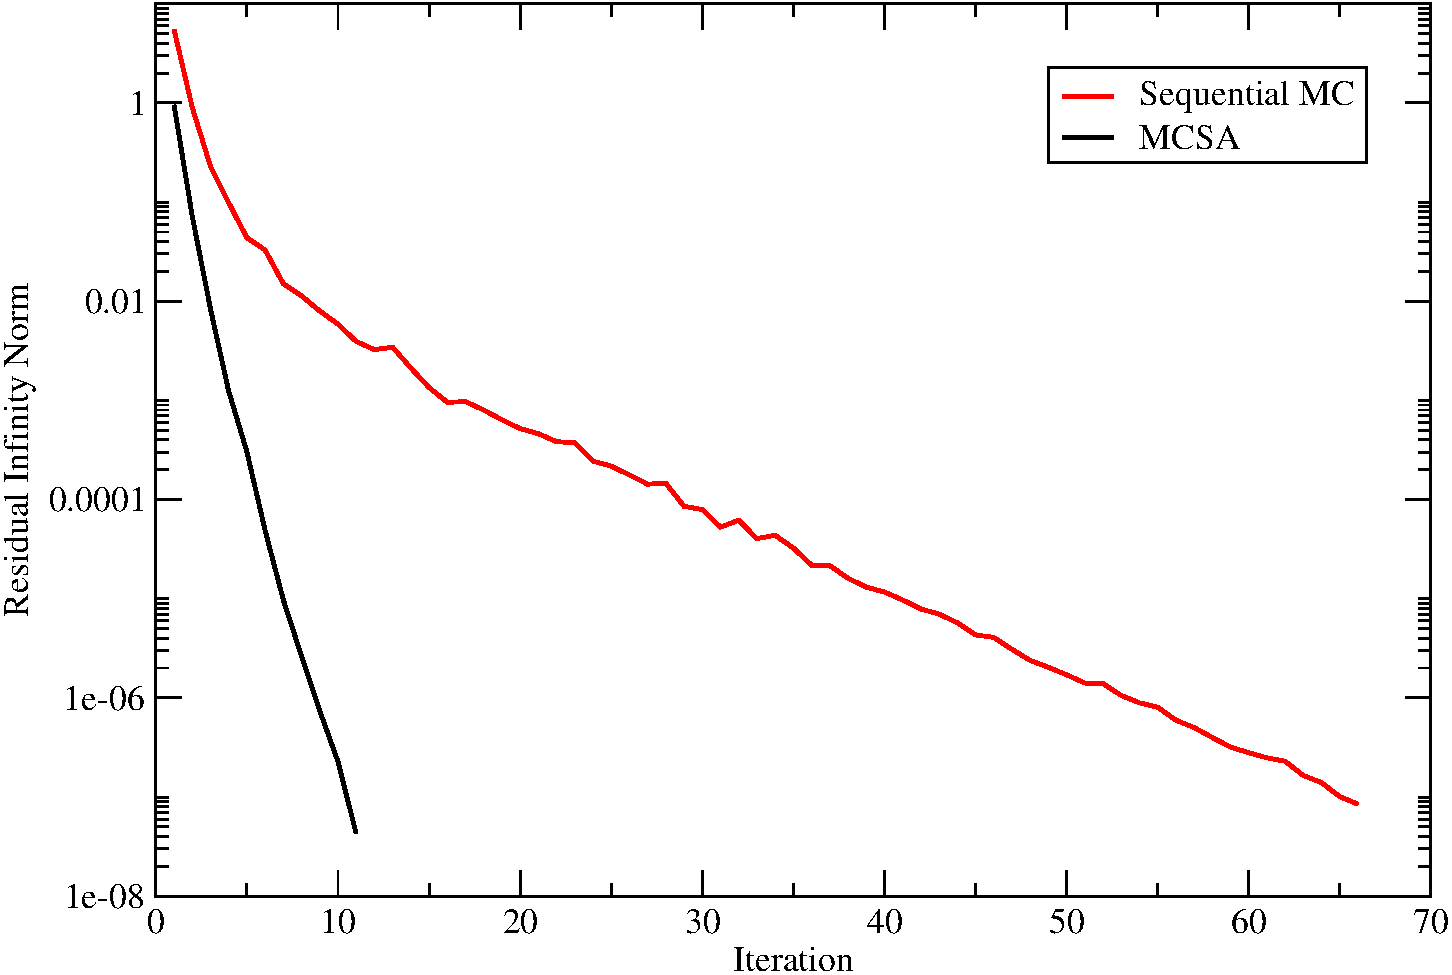
\includegraphics[width=4.5in,clip]{chapters/mc_background/seq_conv_100.pdf}
  \caption{\textbf{Infinity norm of the solution residual
      vs. iteration number for a problem of size $N=100$.}
    \textit{Both the Sequential Monte Carlo and MCSA solvers are used
      with the five point stencils and the adjoint Monte Carlo
      solver.}}
  \label{fig:seq_100}
\end{figure}

\begin{figure}[t!]
  \centering
  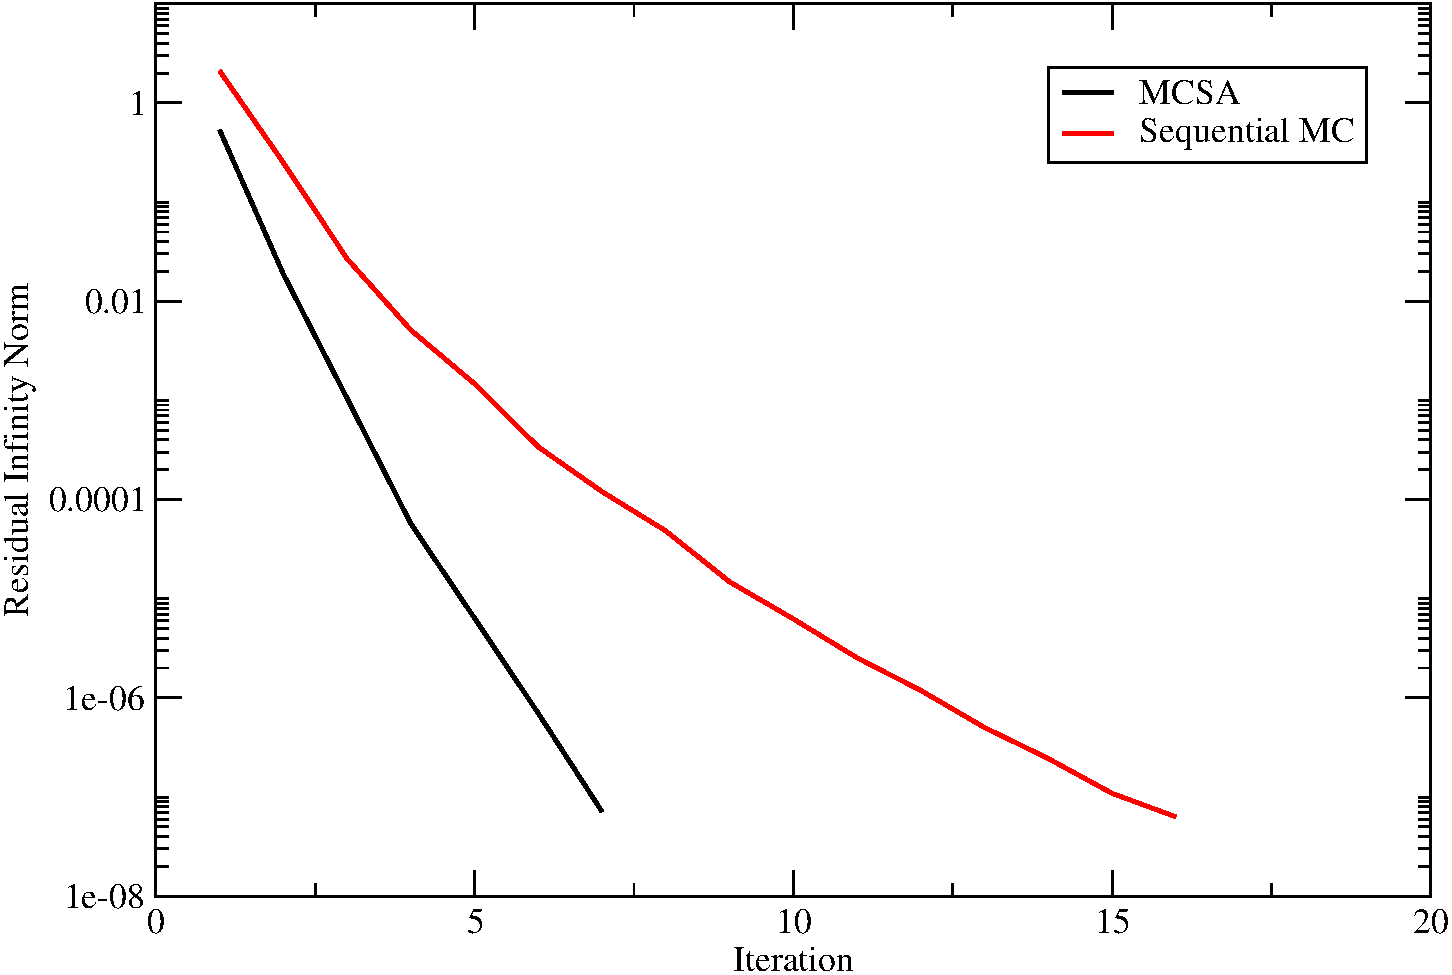
\includegraphics[width=4.5in,clip]{chapters/mc_background/seq_conv_500.pdf}
  \caption{\textbf{Infinity norm of the solution residual
      vs. iteration number for a problem of size $N=500$.}
    \textit{Both the Sequential Monte Carlo and MCSA solvers are used
      with the five point stencils and the adjoint Monte Carlo
      solver.}}
  \label{fig:seq_500}
\end{figure}

\clearpage

\subsection{Monte Carlo Parameter and Estimator Analysis}
\label{sec:parameter_estimator_analysis}
We now study the effects of the adjoint Monte Carlo parameters, weight
cutoff and number of histories, on MCSA performance with both the
collision and expected value estimators. With the same Poisson
problem, we will use a $200 \times 200$ grid and a convergence
tolerance of \sn{1}{-8} for all calculations. To study the effects of
the number of Monte Carlo histories per MCSA iteration, the weight
cutoff was fixed at \sn{1}{-4} while the number of histories per
iteration was varied from 6,000 to 100,000. It was observed that MCSA
would not converge for this problem using the collision estimator with
less than 6,000 histories while the expected value estimator permitted
convergence with only 2,000 histories.

Figure~\ref{fig:estimator_nh_iters} gives the number of iterations
required to converge for both estimators as a function of the number
of histories per iteration. For smaller numbers of histories, the
performance of the expected value estimator is significantly better
than the collision estimator. This result is valuable in that less
transport is required to achieve the same MCSA iterative performance
with the expected value estimator, important for situations where
transport is expensive (i.e. in domain decomposed
calculations). Interestingly, as the number of histories per iteration
are increased, the iterative performance with the collision estimator
approaches that of the expected value estimator. However, given the
performance of the expected value estimator at a fractional number of
histories, one should strongly consider its use over using the
collision estimator with more histories. The CPU time required to
converge is presented in Figure~\ref{fig:estimator_nh_time} and
reflects the results of the iterative performance. In general, using
the collision estimator is slightly slower overall, but the time per
iteration is faster due to the fact that the estimator does not have
to cycle through multiple states during the tally procedure.

\begin{figure}[t!]
  \centering
  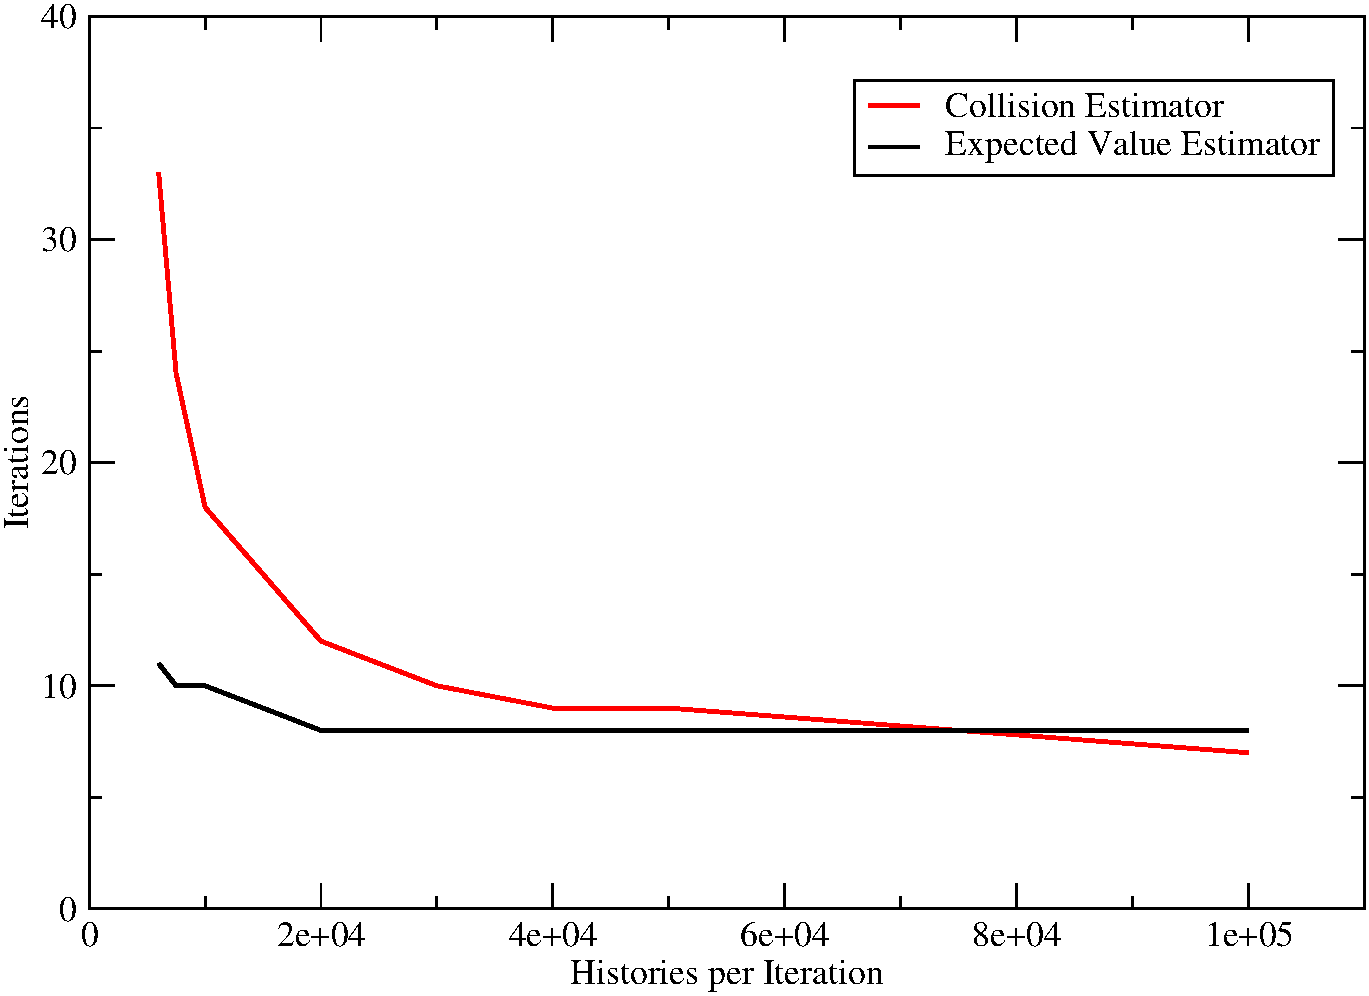
\includegraphics[width=4.75in,clip]{chapters/mc_background/estimator_nh_iters.pdf}
  \caption{\textbf{Iterations (s) to converge vs. Monte Carlo
      histories per MCSA iteration for a $200 \times 200$ square mesh
      and a weight cutoff of \sn{1}{-4}.} \textit{For low numbers of
      histories, the expected value estimator performance is
      significantly better than the collision estimator. At higher
      numbers of histories, the estimators become roughly
      equivalent.}}
  \label{fig:estimator_nh_iters}
\end{figure}

\begin{figure}[t!]
  \centering
  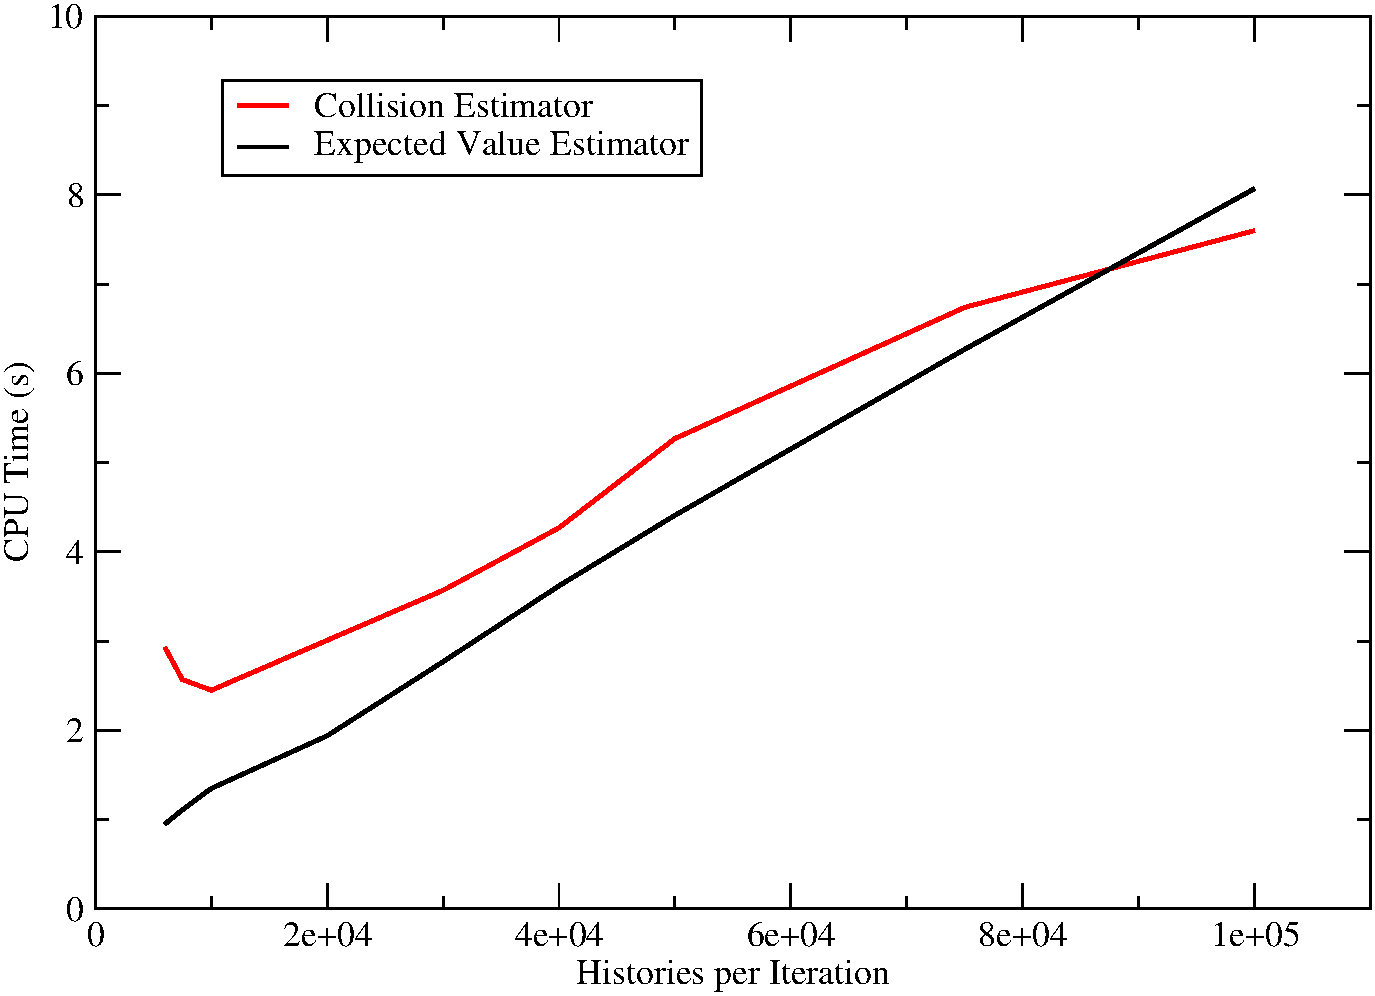
\includegraphics[width=4.75in,clip]{chapters/mc_background/estimator_nh_time.pdf}
  \caption{\textbf{CPU Time (s) to converge vs. Monte Carlo histories
      per MCSA iteration for a $200 \times 200$ square mesh and a
      weight cutoff of \sn{1}{-4}.} \textit{For low numbers of
      histories, the expected value estimator performance is better
      than the collision estimator due to a lower iteration count
      while the actual compute time per iteration is higher.}}
  \label{fig:estimator_nh_time}
\end{figure}

For the weight cutoff study, the number of histories per iteration was
fixed at 40,000 and the weight cutoff varied from \sn{5}{-1} down to
\sn{1}{-10}. Surprisingly, the number of iterations to converge given
by Figure~\ref{fig:estimator_wc_iters} is effectively invariant to the
weight cutoff, only seeing detrimental effects on the number of
iterations at a very large weight cutoff. This suggests that a fairly
large weight cutoff can be used in practice with both adjoint
estimators and that the preliminary components of the random walk are
more important to MCSA convergence than those that occur later and
with lower weight contributions. To further motivate using a larger
weight cutoff, Figure~\ref{fig:estimator_wc_time} gives the CPU time
need to converge as a function of weight cutoff. As expected, lowering
the weight cutoff lengthens the random walk lengths and increases CPU
time at no gain of iterative performance. In general, these results
suggest using the expected value estimator over the collision
estimator with MCSA as well as using a larger weight cutoff.

\begin{figure}[t!]
  \centering
  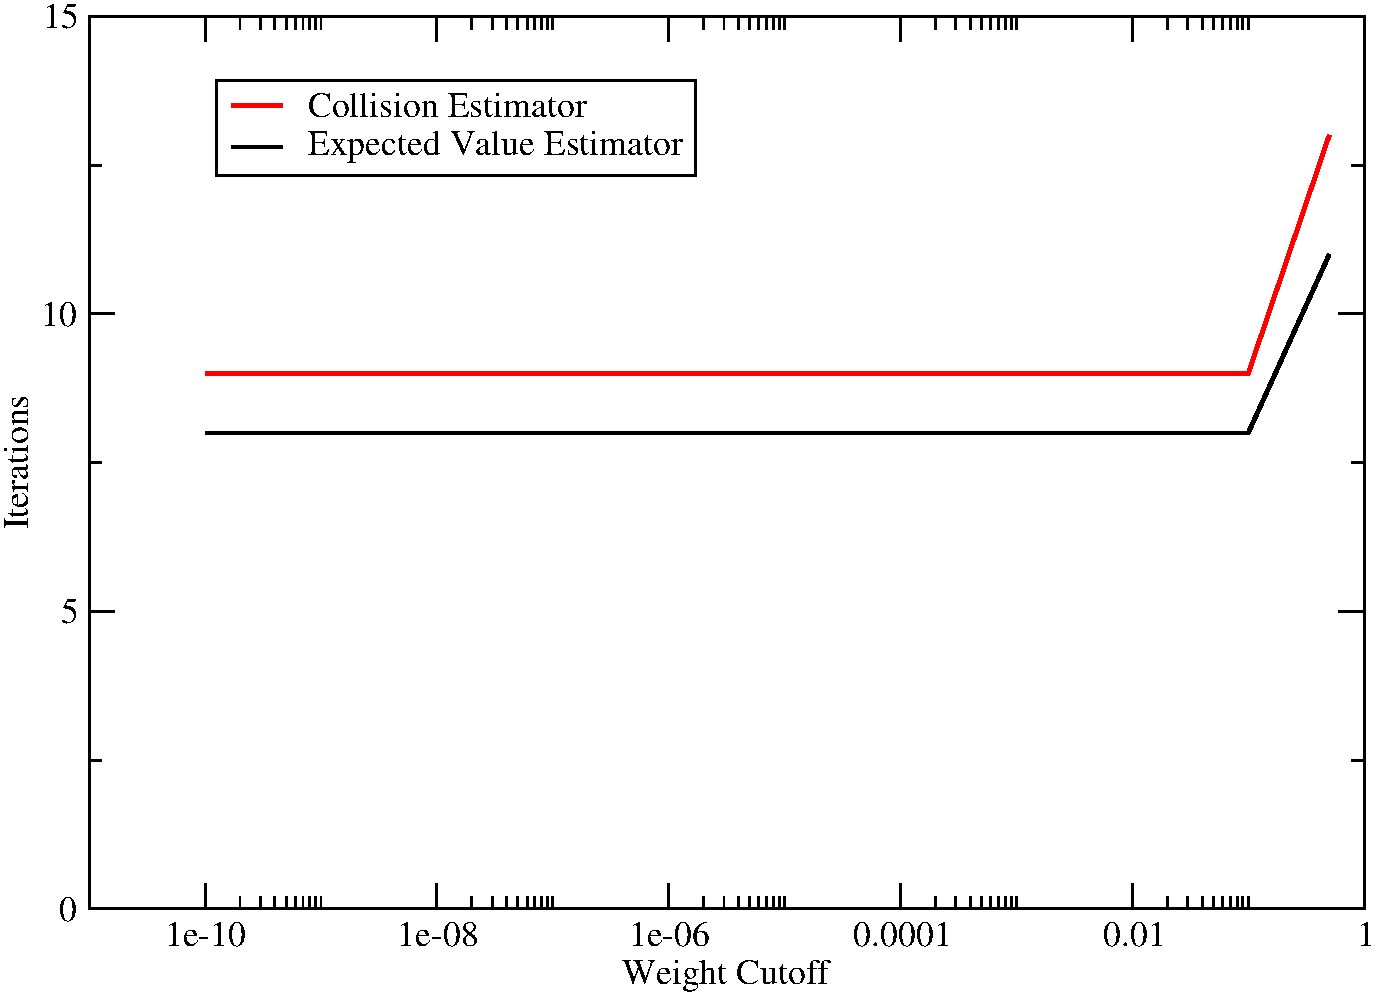
\includegraphics[width=4.75in,clip]{chapters/mc_background/estimator_wc_iters.pdf}
  \caption{\textbf{Iterations (s) to converge vs. history weight
      cutoff for a $200 \times 200$ square mesh and 40,000 histories.}
    \textit{For low numbers of histories, the expected value estimator
      performance is significantly better than the collision
      estimator. At higher numbers of histories, the estimators become
      roughly equivalent.}}
  \label{fig:estimator_wc_iters}
\end{figure}

\begin{figure}[t!]
  \centering
  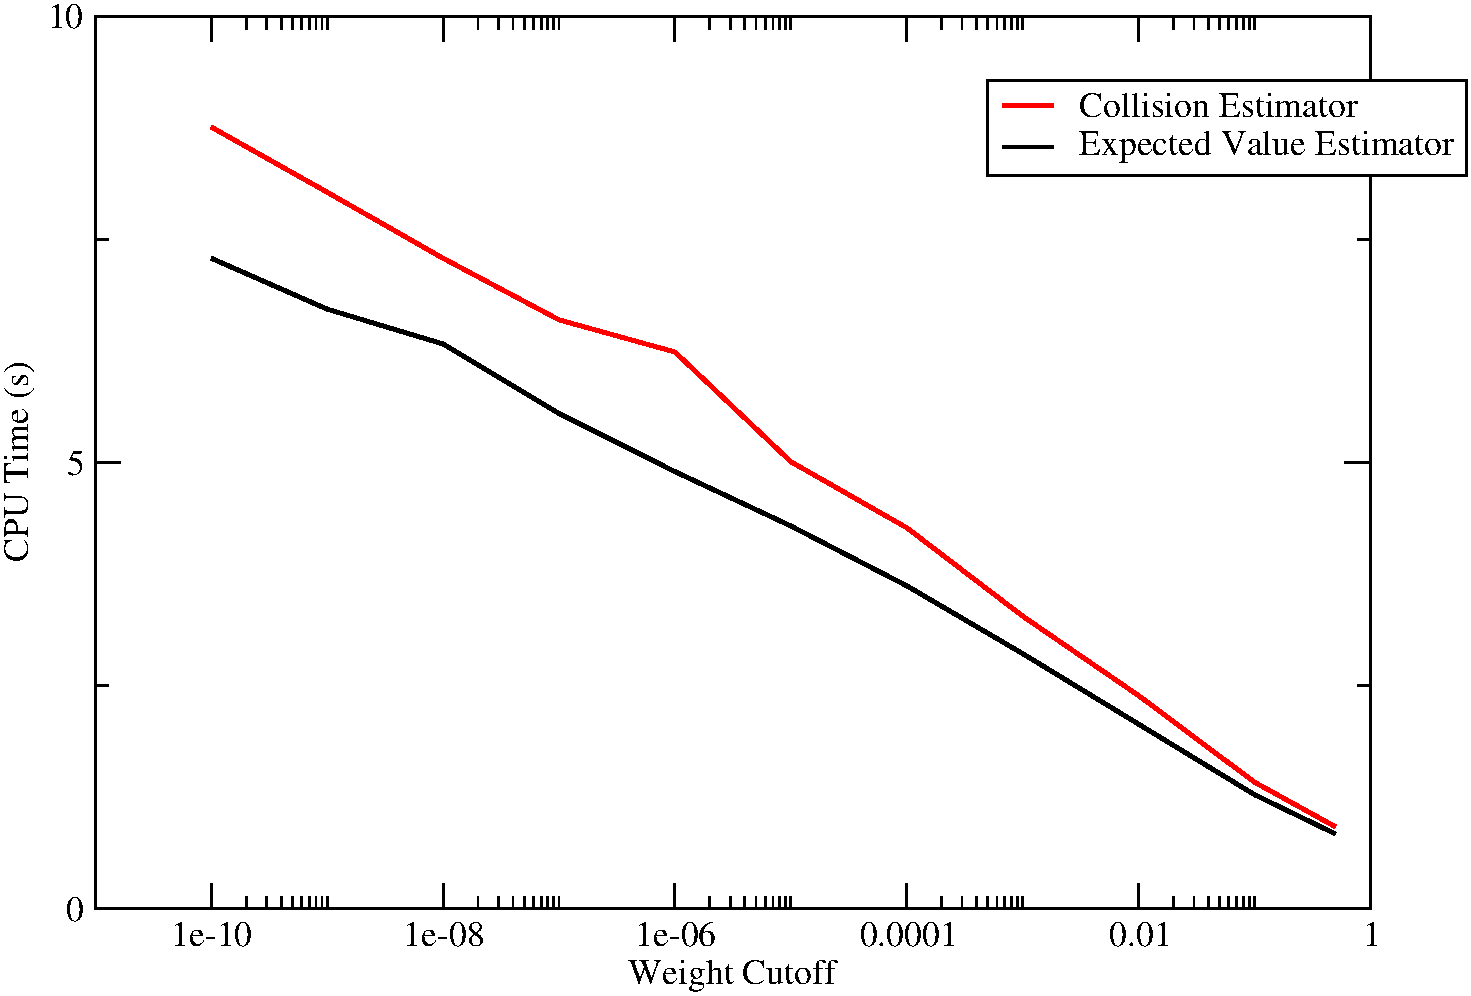
\includegraphics[width=4.75in,clip]{chapters/mc_background/estimator_wc_time.pdf}
  \caption{\textbf{CPU Time (s) to converge vs. history weight cutoff
      for a $200 \times 200$ square mesh and 40,000 histories.}
    \textit{For low numbers of histories, the expected value estimator
      performance is better than the collision estimator due to a
      lower iteration count while the actual compute time per
      iteration is higher.}}
  \label{fig:estimator_wc_time}
\end{figure}

\clearpage

%%---------------------------------------------------------------------------%%
\section{Summary}
\label{sec:mc_summary}

In this chapter, the fundamentals of Monte Carlo Synthetic
Acceleration methods were presented and explored in the context of a
simple model transport system. The following are the significant
observations, findings, and contributions.

\begin{itemize}
\item Monte Carlo Synthetic Acceleration (MCSA) has been generalized
  for all discrete linear transport problems
\item MCSA can be preconditioned using a general left/right scheme but
  requires the explicit inversion of the preconditioners and
  construction of the composite linear operator
\item The adjoint Neumann-Ulam method performs better when used with
  MCSA compared to the forward method
\item MCSA has superior performance when compared to Halton's residual
  Monte Carlo method
\item The Richardson iteration in MCSA behaves as a smoother for the
  stochastic Monte Carlo error
\item MCSA iterative performance when used with the expected value
  estimator is insensitive to histories per iteration
\item MCSA iterative performance is insensitive to the stochastic
  history weight cutoff
\end{itemize}
